\documentclass[aspectratio=169]{beamer}
\usetheme[theme=blue,logo=hustwithtext]{HUST} 

\usepackage[T5]{fontenc}
\usepackage[utf8]{inputenc}
\usepackage{amsmath}
\usepackage{amsfonts}
\usepackage{amssymb}
\usepackage{graphicx}
\usepackage{xcolor}
\usepackage{tikz}
\usepackage{minted}
\usepackage{booktabs} 
\usetikzlibrary{decorations.pathreplacing}
\usetikzlibrary{shapes.arrows, positioning, calc, shapes.multipart, matrix, fit, backgrounds, arrows.meta, trees, shadows, shapes.geometric}

\newcommand{\drawground}[1]{
    \draw[thick] (#1) -- ++(0,-0.3) coordinate(g);
    \draw[thick] ($(g)+(-0.2,0)$) -- ($(g)+(0.2,0)$);
}
\setminted{
    breaklines=true,      % Vẫn cho phép xuống dòng
    breaksymbolleft={},   % Xóa mũi tên ở đầu dòng tiếp theo (quan trọng)
    breaksymbol={},       % Xóa mũi tên ở cuối dòng trước (nếu có)
}
\setminted{
    fontsize=\scriptsize, % Chữ code nhỏ lại chút cho vừa
    baselinestretch=1.0,
    breaklines=true,
    mathescape=false, % QUAN TRỌNG: Tắt chế độ toán học để không lỗi với dấu "_"
    escapeinside=     % Tắt escape để tránh xung đột ký tự lạ
}

% --- Colors ---
\definecolor{bstgreen}{RGB}{112, 173, 71}
\definecolor{pathblue}{RGB}{0, 51, 102}
\definecolor{pathred}{RGB}{192, 0, 0}

\definecolor{textdark}{RGB}{0, 32, 96}
\definecolor{nodered}{RGB}{192, 0, 0}
\definecolor{nodeblue}{RGB}{68, 114, 196}   % Xanh dương cho node
\definecolor{textred}{RGB}{255, 0, 0}       % Đỏ
\definecolor{textpink}{RGB}{255, 0, 255}    % Hồng tím (cho 37)
\definecolor{textorange}{RGB}{255, 102, 0}  % Cam (cho 53)

\definecolor{HUSTBlue}{RGB}{0,51,102}
\definecolor{HUSTRed}{RGB}{192,32,52}
\definecolor{codeblue}{RGB}{0,90,200}
\definecolor{codegreen}{RGB}{0,150,0}
\definecolor{textpurple}{RGB}{255, 0, 255}
\definecolor{slashpink}{RGB}{255, 0, 255}
\definecolor{arrowblue}{RGB}{200, 230, 255}
\definecolor{arrowyellow}{RGB}{255, 255, 204} % Vàng nhạt mũi tên
\definecolor{triangleblue}{RGB}{0, 112, 192} % Xanh tam giác
% --- TikZ Styles ---

\definecolor{nodefill}{RGB}{245, 245, 220} % Màu kem nhạt cho nền node
\definecolor{nodetext}{RGB}{100, 160, 60}  % Màu xanh lá cho chữ và viền
\definecolor{edgeorange}{RGB}{240, 140, 60} % Màu cam cho cạnh
\definecolor{pathblue}{RGB}{40, 40, 180}   % Màu xanh dương cho đường duyệt
\definecolor{resultred}{RGB}{200, 0, 0}    % Màu đỏ cho kết quả
\tikzset{
    arraynode/.style={
        draw, minimum size=0.8cm, fill=white, anchor=center
    },
    treenode/.style={
        circle, draw, fill=blue!10, minimum size=0.8cm, inner sep=0pt
    },
    ptr/.style={
        ->, >=stealth, thick, HUSTRed
    },
    labelptr/.style={
        font=\footnotesize, color=HUSTBlue
    }
}

% --- Minted Settings ---
\setminted{
    breaklines=true,
    autogobble=true,
    tabsize=4,
    linenos=true,
    fontsize=\scriptsize,
    frame=single,
    rulecolor=\color{black!30},
    baselinestretch=1.0,
}

% --- Content Helper ---
\newcommand{\placecontent}[4]{%
    \tikz[remember picture,overlay]
    \node[anchor=north west]
    at ([xshift=#1,yshift=-#2]current page.north west)
    {\parbox{#3}{#4}};
}
\newcommand{\drawleaf}[2]{
    \draw[thick] (#1) -- ++(#2:0.7) coordinate (leaf);
    \draw[thick] ($(leaf)+({#2+90}:0.2)$) -- ($(leaf)+({#2-90}:0.2)$);
}

% =========================================================
% INFO
% =========================================================
\title{\huge CẤU TRÚC DỮ LIỆU VÀ GIẢI THUẬT}
\subtitle{Tìm kiếm & Cây nhị phân tìm kiếm}
\author{SoICT - HUST}
\date{\today}

\begin{document}

% --- Cover Slides ---
\HUSTInsertBrandSlide
\HUSTInsertThemeSlide

% --- Title Slide ---
{\HUSTUseBackground{onelove.pdf}
\begin{frame}
    \ifdefstring{\insertaspectratio}{169}{
        \HUSTCornerImage[0.14]{assets/logo/soict_vi_h.pdf}
        \placecontent{0.5cm}{0.33\paperheight}{0.85\paperwidth}{
            \color{\HUSTFrameTitleTextColor}\bfseries\fontsize{22pt}{30pt}\selectfont
            \inserttitle
        }
        \placecontent{0.5cm}{0.50\paperheight}{0.8\paperwidth}{
            \color{\HUSTFrameTitleTextColor}\fontsize{14pt}{14pt}\selectfont
            \textbf{\large TUẦN 11: Tìm kiếm Tuần tự, Nhị phân \& BST}\\
        }
    }{}
\end{frame}
}

% --- TOC ---
\begin{frame}{NỘI DUNG}
    \tableofcontents
\end{frame}

% =========================================================
% 1. LINEAR SEARCH
% =========================================================
\section{Tìm kiếm tuần tự (Linear Search)}
\subsection{Bài toán tìm kiếm}
\begin{frame}[fragile]{1. Tìm kiếm tuần tự}
    \textbf{1.1. Bài toán}
    \begin{itemize}
        \item \textbf{Input:} Danh sách $a$ gồm $n$ phần tử $a_1, a_2, \dots, a_n$ và số $x$.
        \item \textbf{Yêu cầu:} 
        \begin{itemize}
            \item $x$ có mặt trong danh sách không?
            \item Nếu có, hãy đưa ra \textit{\color{HUSTBlue} vị trí xuất hiện của x trong dãy đã cho}
            \begin{itemize}
                \item chỉ số $i$ sao cho $a_i = x$.
            \end{itemize}
        \end{itemize} 
    \end{itemize}
\end{frame}
\subsection{Giải thuật}
\begin{frame}[fragile]{1. TÌm kiếm tuần tự}
    \textbf{1.2. Giải thuật}
    \begin{itemize}
        \item Bắt đầu từ phần tử đầu tiên, duyệt qua từng phần tử cho đến khi tìm được
đích hoặc kết luận không tìm được.
        \item Các số không cần sắp thứ tự
        \item Làm việc được với cả danh sách móc nối (Linked Lists)
        \item \textbf{Độ phức tạp:} $O(n)$.
    \end{itemize}
    \begin{columns}
        \begin{column}{0.55\textwidth}
            \begin{minted}{c}
int linearSearch(float a[], int size, float x) {
    int i;
    for (i = 0; i < size; i++) {
        if (a[i] == x) {
            return i; // Tìm thấy
        }
    }
    return -1; // Không tìm thấy
}
            \end{minted}
        \end{column}
        \begin{column}{0.45\textwidth}
            \centering
            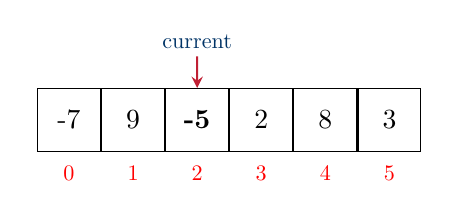
\begin{tikzpicture}[scale=0.8, transform shape]
                \matrix[matrix of nodes, nodes={arraynode}, column sep=0pt] (arr) {
                    -7 & 9 & \textbf{-5} & 2 & 8 & 3 \\
                };
                \node[above=0.5cm of arr-1-3, HUSTBlue] (curr) {current};
                \draw[ptr] (curr) -- (arr-1-3);
                \node[below=0.1cm of arr-1-6, red] {$5$};
                \node[below=0.1cm of arr-1-5, red] {$4$};
                \node[below=0.1cm of arr-1-4, red] {$3$};
                \node[below=0.1cm of arr-1-3, red] {$2$};
                \node[below=0.1cm of arr-1-2, red] {$1$};
                \node[below=0.1cm of arr-1-1, red] {$0$};
            \end{tikzpicture}
        \end{column}
    \end{columns}
\end{frame}

\begin{frame}{1. Tìm kiếm tuần tự}
    \textbf{1.3. Phân tích thời gian tính}
    \begin{itemize}
        \item Độ dài đầu vào: $n$
        \item Đánh giá số lần thực hiện
        \\[0.5em] 
        \hspace{0.6cm} {\color{blue}(*) \quad $\mathbf{(a[i] == x)}$ \quad} trong vòng lặp for.
        
        \vspace{0.5em}
        \item Nếu $a[1] = x$ (phần tử cần tìm ở đầu):
        \begin{itemize}
            \item {\color{blue}(*)} phải thực hiện 1 lần.
            \\ $\rightarrow$ thời gian tính \textcolor{red}{\textbf{tốt nhất}}: $\Theta(1)$.
        \end{itemize}
        
        \vspace{0.5em}
        \item Nếu $x$ không có mặt trong dãy:
        \begin{itemize}
            \item {\color{blue}(*)} phải thực hiện $n$ lần.
            \\ $\rightarrow$ thời gian tính \textcolor{red}{\textbf{tồi nhất}}: $\Theta(n)$.
        \end{itemize}
    \end{itemize}
\end{frame}
% =========================================================
% 2. BINARY SEARCH
% =========================================================
\section{Tìm kiếm nhị phân (Binary Search)}
\subsection{Bài toán}
\begin{frame}{2. Tìm kiếm nhị phân}
    \textbf{2.1. Bài toán}
    \begin{itemize}
        \item Cho mảng $a[1..n]$ đã được \textbf{sắp xếp} theo thứ tự không giảm và số $x$. \\
        Cần tìm chỉ số $i$ ($1 \le i \le n$) sao cho $a[i] = x$.
        \item \textbf{Ý tưởng:} So sánh $x$ với phần tử ở giữa (\texttt{mid}).
        \begin{enumerate}
            \item Nếu $a[mid] = x$: Tìm thấy.
            \item Nếu $x < a[mid]$: Tìm tiếp ở nửa bên trái (Left).
            \item Nếu $x > a[mid]$: Tìm tiếp ở nửa bên phải (Right).
        \end{enumerate}
        \item \textbf{\color{HUSTBlue}Nhận xét: $x$} có trong mảng $a$ thì hoặc là $x$ \\ (1) bằng phần tử nằm ở vị trí ở giữa mảng $a$
        
    \end{itemize}

    \centering
    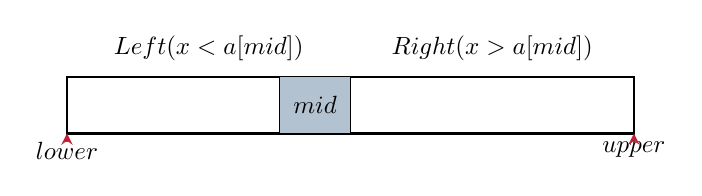
\begin{tikzpicture}[scale=0.9, transform shape]
        \draw[thick] (0,0) rectangle (8, 0.8);
        \draw[fill=HUSTBlue!30] (3,0) rectangle (4, 0.8);
        \node at (3.5, 0.4) {$mid$};
        \node[below] at (0,0) {$lower$};
        \node[below] at (8,0) {$upper$};
        \draw[ptr] (0,-0.1) -- (0,0);
        \draw[ptr] (8,-0.1) -- (8,0);
        
        \node[above] at (2, 0.9) {$Left (x < a[mid])$};
        \node[above] at (6, 0.9) {$Right (x > a[mid])$};
    \end{tikzpicture}
\end{frame}

\begin{frame}{2. Tìm kiếm nhị phân}
    \textbf{2.1. Bài toán}
    \begin{itemize}
        \item Cho mảng $a[1..n]$ đã được \textbf{sắp xếp} theo thứ tự không giảm và số $x$. \\
        Cần tìm chỉ số $i$ ($1 \le i \le n$) sao cho $a[i] = x$.
        
        \item \textbf{\color{HUSTBlue}Nhận xét: $x$} có trong mảng $a$ thì hoặc là $x$ \\ (2) nằm ở nửa bên trái (L) của mảng $a$
        
    \end{itemize}

    \centering
    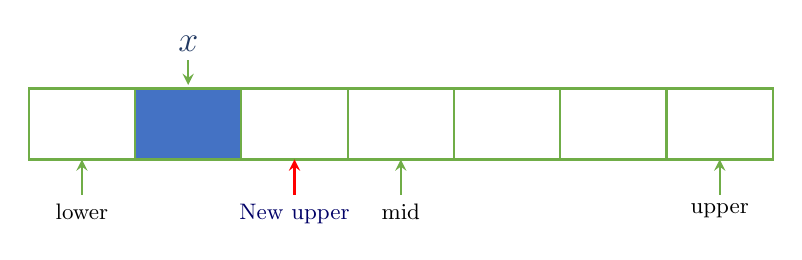
\begin{tikzpicture}[scale=0.9, transform shape] 
    % Định nghĩa màu sắc
    \definecolor{mygreen}{RGB}{112, 173, 71}
    \definecolor{myblue}{RGB}{68, 114, 196}
    \definecolor{myred}{RGB}{255, 0, 0}

    % 1. Vẽ các ô của mảng (7 ô) - Chiều rộng mỗi ô là 1.5
    \foreach \x in {0,...,6} {
        \draw[thick, draw=mygreen] (\x*1.5, 0) rectangle (\x*1.5 + 1.5, 1);
    }

    % 2. Tô màu ô chứa x (vị trí index 1)
    \fill[myblue] (1.5, 0) rectangle (3.0, 1);
    \draw[thick, draw=mygreen] (1.5, 0) rectangle (3.0, 1); 

    % 3. Vẽ mũi tên và nhãn cho x (ở trên)
    \node[above, text=myblue!50!black] at (2.25, 1.4) {\Large $x$};
    \draw[->, >=stealth, thick, mygreen] (2.25, 1.4) -- (2.25, 1.05);

    % 4. Các biến chỉ số (ở dưới)
    % Biến lower (Index 0)
    \draw[->, >=stealth, thick, mygreen] (0.75, -0.5) node[below, black] {\small lower} -- (0.75, 0);

    % Biến New upper (Index 2) - Mũi tên đỏ
    \draw[->, >=stealth, thick, myred] (3.75, -0.5) node[below, text=blue!40!black] {\small New upper} -- (3.75, 0);
    % Biến mid (Index 3)
    \draw[->, >=stealth, thick, mygreen] (5.25, -0.5) node[below, black] {\small mid} -- (5.25, 0);

    % Biến upper (Index 6)
    \draw[->, >=stealth, thick, mygreen] (9.75, -0.5) node[below, black] {\small upper} -- (9.75, 0);

\end{tikzpicture}   
\end{frame}

\begin{frame}{2. Tìm kiếm nhị phân}
    \textbf{2.1. Bài toán}
    \begin{itemize}
        \item Cho mảng $a[1..n]$ đã được \textbf{sắp xếp} theo thứ tự không giảm và số $x$. \\
        Cần tìm chỉ số $i$ ($1 \le i \le n$) sao cho $a[i] = x$.
        
        \item \textbf{\color{HUSTBlue}Nhận xét: $x$} có trong mảng $a$ thì hoặc là $x$ \\ (3) nằm ở nửa bên phải (R) của mảng $a$.
        
    \end{itemize}

    \centering
    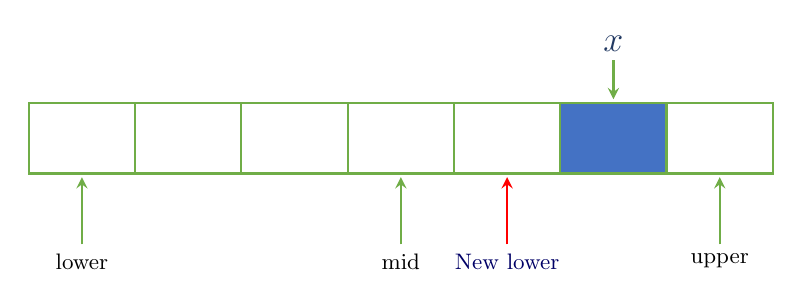
\begin{tikzpicture}[scale=0.9, transform shape]
    % Định nghĩa màu sắc
    \definecolor{mygreen}{RGB}{112, 173, 71}
    \definecolor{myblue}{RGB}{68, 114, 196}
    \definecolor{myred}{RGB}{255, 0, 0}

    % 1. Vẽ các ô của mảng (7 ô) - Chiều rộng mỗi ô là 1.5
    \foreach \x in {0,...,6} {
        \draw[thick, draw=mygreen] (\x*1.5, 0) rectangle (\x*1.5 + 1.5, 1);
    }

    % 2. Tô màu ô chứa x (vị trí index 5 - ô thứ 6)
    % Tọa độ x bắt đầu từ 5*1.5 = 7.5 đến 9.0
    \fill[myblue] (7.5, 0) rectangle (9.0, 1);
    \draw[thick, draw=mygreen] (7.5, 0) rectangle (9.0, 1); % Vẽ lại viền

    % 3. Vẽ mũi tên và nhãn cho x (ở trên)
    % Vị trí giữa ô index 5 là 7.5 + 0.75 = 8.25
    \node[above, text=myblue!50!black] at (8.25, 1.6) {\Large $x$};
    \draw[->, >=stealth, thick, mygreen] (8.25, 1.6) -- (8.25, 1.05);

    % 4. Các biến chỉ số (ở dưới) - y = -1.0
    
    % Biến lower (Index 0) - Vị trí cũ
    \draw[->, >=stealth, thick, mygreen] (0.75, -1.0) node[below, black] {\small lower} -- (0.75, -0.05);

    % Biến mid (Index 3) - Vị trí cũ
    \draw[->, >=stealth, thick, mygreen] (5.25, -1.0) node[below, black] {\small mid} -- (5.25, -0.05);

    % Biến New lower (Index 4) - Mũi tên đỏ mới
    % Vì x > a[mid], vùng tìm kiếm sang phải => lower mới = mid + 1 (index 4)
    % Vị trí giữa ô index 4 là 4*1.5 + 0.75 = 6.75
    \draw[->, >=stealth, thick, myred] (6.75, -1.0) node[below, text=blue!40!black] {\small New lower} -- (6.75, -0.05);

    % Biến upper (Index 6) - Vị trí cũ
    \draw[->, >=stealth, thick, mygreen] (9.75, -1.0) node[below, black] {\small upper} -- (9.75, -0.05);

\end{tikzpicture}
\end{frame}
\subsection{Ví dụ}
\begin{frame}{2. Tìm kiếm nhị phân}
\textbf{2.1. Bài toán}
\begin{itemize}
    \item Cho mảng số $a[1..n]$ được sắp xếp theo thứ tự không giảm và số $x$. \\
    Cần tìm chỉ số $i$ ($1 \le i \le n$) sao cho $a[i] = x$.
    
    \item \textcolor{blue}{Nhận xét:} % Hoặc dùng màu HUSTBlue nếu đã định nghĩa
    \begin{itemize}
        \item Tình huống (2) và (3) xảy ra chỉ khi $x$ nhỏ hơn (lớn hơn) phần tử ở giữa của mảng $a$.
        \item $\rightarrow$ Lặp lại tìm $x$ ở nửa (L) hoặc (R)
    \end{itemize}
\end{itemize}
\end{frame}

\begin{frame}{2. Tìm kiếm nhị phân} % Tiêu đề frame (tùy chỉnh)

    \textbf{2.2. Ví dụ}
    \begin{itemize}
        \item Cho mảng $a = \{1, 3, 4, 7, 8, 9, 12\}$ tìm số $x = 8$
    \end{itemize}

    \vspace{0.5cm} % Tạo khoảng cách

    \begin{center}
    \begin{tikzpicture}[scale=0.9, transform shape]
        % Định nghĩa màu sắc (theo theme HUST/hình ảnh)
        \definecolor{mygreen}{RGB}{112, 173, 71}
        \definecolor{myblue}{RGB}{0, 32, 96} % Xanh đậm cho chữ "Mảng a"
        \definecolor{myred}{RGB}{255, 0, 0}

        % Nhãn "Mảng a" bên trái
        \node[text=myblue, font=\bfseries] at (-1.5, 0.5) {Mảng a};

        % 1. Vẽ các ô của mảng và điền số
        % Mảng giá trị: 1, 3, 4, 7, 8, 9, 12
        \foreach \val [count=\i from 0] in {1, 3, 4, 7, 8, 9, 12} {
            % Vẽ ô chữ nhật (rộng 1.5, cao 1)
            \draw[thick, draw=mygreen] (\i*1.5, 0) rectangle (\i*1.5 + 1.5, 1);
            % Điền số vào giữa ô
            \node[text=mygreen!80!black, font=\large] at (\i*1.5 + 0.75, 0.5) {\val};
        }

        % 2. Các biến chỉ số (lower, mid, upper)
        % Mũi tên hướng TỪ chữ LÊN ô
        
        % lower (Index 0) - Tâm tại 0.75
        \node[below, text=myblue] (lbl_lower) at (0.75, -0.8) {\small lower};
        \draw[->, >=stealth, thick, mygreen] (lbl_lower.north) -- (0.75, -0.05);

        % mid (Index 3) - Tâm tại 3*1.5 + 0.75 = 5.25
        \node[below, text=myblue] (lbl_mid) at (5.25, -0.8) {\small mid};
        \draw[->, >=stealth, thick, mygreen] (lbl_mid.north) -- (5.25, -0.05);

        % upper (Index 6) - Tâm tại 6*1.5 + 0.75 = 9.75
        \node[below, text=myblue] (lbl_upper) at (9.75, -0.8) {\small upper};
        \draw[->, >=stealth, thick, mygreen] (lbl_upper.north) -- (9.75, -0.05);

        % 3. Dấu ngoặc nhọn (Braces)
        % Brace (L): Từ đầu mảng đến sát mid (Index 0-2)
        % Tọa độ x: 0 đến 3*1.5 = 4.5
        \draw [decorate, decoration={brace, amplitude=5pt, mirror, raise=4pt}, thick] 
            (0, -1.3) -- (4.5, -1.3) node [black, midway, yshift=-0.6cm] {\small (L)};

        % Brace (R): Từ sau mid đến cuối mảng (Index 4-6)
        % Tọa độ x: 4*1.5 = 6.0 đến 7*1.5 = 10.5
        \draw [decorate, decoration={brace, amplitude=5pt, mirror, raise=4pt}, thick] 
            (6.0, -1.3) -- (10.5, -1.3) node [black, midway, yshift=-0.6cm] {\small (R)};

        % 4. Hộp kết luận (x != a[mid])
        % Vẽ hộp màu đỏ ở dưới cùng
        \node[draw=red, thick, inner sep=5pt, font=\Large] at (5.25, -3.0) {x != $a[mid]$};

    \end{tikzpicture}
    \end{center}
\end{frame}

\begin{frame}{2. Tìm kiếm nhị phân}

    \textbf{2.2. Ví dụ}
    \begin{itemize}
        \item Cho mảng $a = \{1, 3, 4, 7, 8, 9, 12\}$ tìm số $x = 8$
    \end{itemize}

    \vspace{0.5cm}

    \begin{center}
    \begin{tikzpicture}[scale=0.9, transform shape]
        % Định nghĩa màu sắc
        \definecolor{mygreen}{RGB}{112, 173, 71}
        \definecolor{myblue}{RGB}{0, 32, 96} % Xanh đậm
        \definecolor{myred}{RGB}{255, 0, 0}

        % Nhãn "Mảng a" bên trái
        \node[text=myblue, font=\bfseries] at (-1.5, 0.5) {Mảng a};

        % 1. Vẽ các ô của mảng và điền số
        \foreach \val [count=\i from 0] in {1, 3, 4, 7, 8, 9, 12} {
            \draw[thick, draw=mygreen] (\i*1.5, 0) rectangle (\i*1.5 + 1.5, 1);
            \node[text=mygreen!80!black, font=\large] at (\i*1.5 + 0.75, 0.5) {\val};
        }

        % 2. Các biến chỉ số (lower, mid, upper)
        % lower (Index 0) - Tâm tại 0.75
        \node[below, text=myblue] (lbl_lower) at (0.75, -0.8) {\small lower};
        \draw[->, >=stealth, thick, mygreen] (lbl_lower.north) -- (0.75, -0.05);

        % mid (Index 3) - Tâm tại 3*1.5 + 0.75 = 5.25
        \node[below, text=myblue] (lbl_mid) at (5.25, -0.8) {\small mid};
        \draw[->, >=stealth, thick, mygreen] (lbl_mid.north) -- (5.25, -0.05);

        % New lower (Index 4) - Mũi tên đỏ
        % Tâm tại 4*1.5 + 0.75 = 6.75
        \node[below, text=myblue] (lbl_new) at (6.75, -0.8) {\small New lower};
        \draw[->, >=stealth, thick, myred] (lbl_new.north) -- (6.75, -0.05);

        % upper (Index 6) - Tâm tại 6*1.5 + 0.75 = 9.75
        \node[below, text=myblue] (lbl_upper) at (9.75, -0.8) {\small upper};
        \draw[->, >=stealth, thick, mygreen] (lbl_upper.north) -- (9.75, -0.05);

        % 3. Hộp kết luận (x > a[mid])
        % Hộp viền đỏ, chữ xanh/đen
        \node[draw=red, thick, inner sep=6pt, font=\Large] at (5.25, -2.5) {$x > a[mid] \rightarrow$ Tìm ở nửa bên phải};

    \end{tikzpicture}
    \end{center}
\end{frame}

\begin{frame}{2. Tìm kiếm nhị phân}

    \textbf{2.2. Ví dụ}
    \begin{itemize}
        \item Cho mảng $a = \{1, 3, 4, 7, 8, 9, 12\}$ tìm số $x = 8$
    \end{itemize}

    \vspace{0.5cm}

    \begin{center}
    \begin{tikzpicture}[scale=0.9, transform shape]
        % Định nghĩa màu sắc
        \definecolor{mygreen}{RGB}{112, 173, 71}
        \definecolor{myblue}{RGB}{0, 32, 96}
        \definecolor{myred}{RGB}{255, 0, 0}

        % Nhãn "Mảng a"
        \node[text=myblue, font=\bfseries] at (-1.5, 0.5) {Mảng a};

        % 1. Vẽ các ô của mảng và điền số
        \foreach \val [count=\i from 0] in {1, 3, 4, 7, 8, 9, 12} {
            \draw[thick, draw=mygreen] (\i*1.5, 0) rectangle (\i*1.5 + 1.5, 1);
            \node[text=mygreen!80!black, font=\large] at (\i*1.5 + 0.75, 0.5) {\val};
        }

        % 2. Các biến chỉ số (lower, mid, upper)
        
        % lower (Index 4) - Tâm tại 4*1.5 + 0.75 = 6.75
        \node[below, text=myblue] (lbl_lower) at (6.75, -0.8) {\small lower};
        \draw[->, >=stealth, thick, mygreen] (lbl_lower.north) -- (6.75, -0.05);

        % mid (Index 5) - Tâm tại 5*1.5 + 0.75 = 8.25
        \node[below, text=myblue] (lbl_mid) at (8.25, -0.8) {\small mid};
        \draw[->, >=stealth, thick, mygreen] (lbl_mid.north) -- (8.25, -0.05);

        % upper (Index 6) - Tâm tại 6*1.5 + 0.75 = 9.75
        \node[below, text=myblue] (lbl_upper) at (9.75, -0.8) {\small upper};
        \draw[->, >=stealth, thick, mygreen] (lbl_upper.north) -- (9.75, -0.05);

        % 3. Dấu ngoặc nhọn (Braces)
        % Brace (L): Dưới ô index 4 (x từ 6.0 đến 7.5)
        \draw [decorate, decoration={brace, amplitude=5pt, mirror, raise=4pt}, thick] 
            (6.0, -1.3) -- (7.5, -1.3) node [black, midway, yshift=-0.6cm] {\small (L)};

        % Brace (R): Dưới ô index 6 (x từ 9.0 đến 10.5)
        \draw [decorate, decoration={brace, amplitude=5pt, mirror, raise=4pt}, thick] 
            (9.0, -1.3) -- (10.5, -1.3) node [black, midway, yshift=-0.6cm] {\small (R)};

        % 4. Hộp kết luận (x < a[mid])
        \node[draw=red, thick, inner sep=6pt, font=\Large] at (5.25, -2.8) {$x < a[mid] \rightarrow$ Tìm ở nửa bên trái};

    \end{tikzpicture}
    \end{center}
\end{frame}

\begin{frame}{2. Tìm kiếm nhị phân}

    \textbf{2.2. Ví dụ}
    \begin{itemize}
        \item Cho mảng $a = \{1, 3, 4, 7, 8, 9, 12\}$ tìm số $x = 8$
    \end{itemize}

    \vspace{0.5cm}

    \begin{center}
    \begin{tikzpicture}[scale=1.0, transform shape]
        % Định nghĩa màu sắc
        \definecolor{mygreen}{RGB}{112, 173, 71}
        \definecolor{myblue}{RGB}{0, 32, 96}
        \definecolor{myred}{RGB}{255, 0, 0}

        % Nhãn "Mảng a"
        \node[text=myblue, font=\bfseries] at (-1.5, 0.5) {Mảng a};

        % 1. Vẽ các ô của mảng và điền số
        % Mảng giá trị: 1, 3, 4, 7, 8, 9, 12
        \foreach \val [count=\i from 0] in {1, 3, 4, 7, 8, 9, 12} {
            \draw[thick, draw=mygreen] (\i*1.5, 0) rectangle (\i*1.5 + 1.5, 1);
            \node[text=mygreen!80!black, font=\large] at (\i*1.5 + 0.75, 0.5) {\val};
        }

        % 2. Các biến chỉ số (lower, mid, upper)
        % Tất cả trỏ vào ô Index 4 (Giá trị 8) - Tọa độ x của ô từ 6.0 đến 7.5
        
        % lower: Dịch hẳn sang trái (x = 6)
        \draw[->, >=stealth, thick, mygreen] (6, -1.0) node[below, black, font=\footnotesize] {lower} -- (6, -0.05);

        % mid: Ở chính giữa (x = 6.75)
        \draw[->, >=stealth, thick, mygreen] (6.75, -1.0) node[below, black, font=\footnotesize] {mid} -- (6.75, -0.05);

        % upper: Dịch hẳn sang phải (x = 7.35) - Mũi tên ĐỎ
        \draw[->, >=stealth, thick, myred] (7.5, -1.0) node[below, black, font=\footnotesize] {upper} -- (7.5, -0.05);

        % 3. Hộp kết luận
        \node[draw=red, thick, inner sep=8pt, font=\Large] at (5.25, -2.5) {$x = a[mid] \rightarrow$ Dừng và đưa ra kết quả};

    \end{tikzpicture}
    \end{center}
\end{frame}
\begin{frame}[fragile]{2. Tìm kiếm nhị phân - Cài đặt}
    \vspace{-1em}
    \begin{columns}[T]
        \begin{column}{0.52\textwidth}
            \textbf{Dùng vòng lặp (Iterative)}
            \begin{minted}[fontsize=\scriptsize]{c}
int binarySearch(float a[], int size, float x){
    int lower = 0, upper = size - 1;
    while (lower <= upper) {
        int mid = (upper + lower) / 2;
        if (a[mid] > x)
            upper = mid - 1;
        else if (a[mid] < x)
            lower = mid + 1;
        else
            return mid; // Found
    }
    return -1;
}
            \end{minted}
            
            \small Đoạn cần khảo sát có
độ dài giảm đi một nửa
sau mỗi lần lặp
        \end{column}
        \begin{column}{0.49\textwidth}
            \textbf{Đệ quy (Recursive)}
            \begin{minted}[fontsize=\scriptsize]{c}
int binarySearch(float a[], int l, int u, float x){
    if (u >= l) {
        int mid = l + (u - l) / 2;
        if (a[mid] == x)
            return mid;
        if (a[mid] > x)
            return binarySearch(a, l, mid-1, x);
        return binarySearch(a, mid+1, u, x);
    }
    return -1;
}
            \end{minted}
            \vspace{0.2cm}
            \textbf{Độ phức tạp:} $O(\log n)$.
        \end{column}
    \end{columns}
\end{frame}
\begin{frame}{2. Tìm kiếm nhị phân}
    \textbf{\Large Nhận xét:}
    \begin{itemize}
    \item Ưu điểm: 
    \begin{enumerate}
        \item Nhanh hơn tìm kiếm tuyến tính, đặc biệt đối với các mảng lớn.
        \item Hiệu quả hơn các thuật toán tìm kiếm khác có độ phức tạp về thời gian tương tự (ví dụ: tìm
kiếm nội suy hoặc tìm kiếm theo cấp số nhân).
        \item Phù hợp để tìm kiếm các tập dữ liệu lớn được lưu trữ trong bộ nhớ ngoài, chẳng hạn như trên ổ
cứng hoặc trên đám mây.
    \end{enumerate}
    \item Nhược điểm: 
    \begin{enumerate}
        \item Mảng nên được sắp xếp.
        \item Yêu cầu cấu trúc dữ liệu đang được tìm kiếm được lưu trữ ở các vị trí bộ nhớ liền kề.
        \item Yêu cầu các phần tử của mảng phải có thể so sánh được, nghĩa là chúng phải có thứ tự.
    \end{enumerate}
    \end{itemize}

\end{frame}

% =========================================================
% 3. BINARY SEARCH TREE (BST)
% =========================================================
\section{Cây nhị phân tìm kiếm (BST)}
\begin{frame}[fragile]{3. Cây nhị phân tìm kiếm (BST)}
    \textbf{3.1. Định nghĩa}\\
    Cây nhị phân có các tính chất sau:
    \begin{itemize}
        \item Cây nhị phân tìm kiếm: cấu trúc dữ liệu quan trọng để biểu diễn tập động, trong đó
tất cả các thao tác đều được thực hiện với thời gian {\color{HUSTBlue}\textit{O(h)}}, trong đó {\color{HUSTBlue}\textit{h là chiều cao
của cây.}}
    \end{itemize}
    \textbf{Mỗi nút x (ngoài thông tin đi kèm) có các trường:}
    \begin{center}
        \begin{tikzpicture}[
            % Định nghĩa style cho Node 4 ngăn
            complexNode/.style={
                rectangle split, 
                rectangle split parts=4,       % Chia làm 4 phần
                rectangle split horizontal,    % Xếp hàng ngang
                draw=HUSTBlue, thick,          % Viền màu
                fill=white,
                minimum height=1cm,          % Chiều cao
                text width=1.1cm,              % Chiều rộng mỗi ngăn
                align=center,                  % Canh giữa chữ
                font=\bfseries\small
            },
            ptr/.style={->, >=stealth, thick, HUSTRed}
        ]

            % --- VẼ NODE 4 NGĂN ---
            \node[complexNode] (N) {
                \nodepart{one} Left           % Ngăn 1
                \nodepart{two} Key            % Ngăn 2
                \nodepart{three} Right        % Ngăn 3
                \nodepart{four} Parent        % Ngăn 4
            };

            % --- VẼ CHÚ THÍCH (Tùy chọn) ---
            % Vẽ các mũi tên chỉ vào từng ngăn để giải thích
            \node[below=1cm of N.one south, font=\scriptsize, color=gray] (t1) {Con trái};
            \draw[->, gray] (t1) -- (N.one south);

            \node[below=1cm of N.two south, font=\scriptsize, color=gray] (t2) {Dữ liệu};
            \draw[->, gray] (t2) -- (N.two south);

            \node[below=1cm of N.three south, font=\scriptsize, color=gray] (t3) {Con phải};
            \draw[->, gray] (t3) -- (N.three south);

            \node[below=1cm of N.four south, font=\scriptsize, color=gray] (t4) {Cha};
            \draw[->, gray] (t4) -- (N.four south);

        \end{tikzpicture}
    \end{center}
\end{frame}

\begin{frame}[fragile]{3. Cây nhị phân tìm kiếm (BST)}
    \textbf{3.1. Định nghĩa}
    \vspace{-3em}
    \begin{columns}
        
        \begin{column}{0.6\textwidth}
            \begin{itemize}
            \item Cây nhị phân tìm kiếm(BST) là cây nhị phân thỏa mãn tính chất với mọi nút $x$:
            \begin{itemize}
                \item Các nút thuộc cây con \textbf{trái} có khoá $< key(x)$.
                \item Các nút thuộc cây con \textbf{phải} có khoá $> key(x)$.
            \end{itemize}
        \end{itemize}            
            \vspace{0.3cm}
            \textbf{Cấu trúc Node:}
            \begin{minted}{c}
struct TreeNodeRec {
    float key;
    struct TreeNodeRec* leftPtr;
    struct TreeNodeRec* rightPtr;
};
typedef struct TreeNodeRec TreeNode;
            \end{minted}
        \end{column}
        \begin{column}{0.35\textwidth}
            \centering
            \vspace{2em}
            \begin{tikzpicture}[
        level distance=1cm,
        sibling distance=2.5cm,
        level 2/.style={sibling distance=1cm},
        nodes={treenode} 
    ]
        % --- QUAN TRỌNG: Đặt tên node gốc là (root) ---
        \node (root) {15} 
            child {node {6}
                child {node {4}}
                child {node {7}}
            }
            child {node {23}
                child {node {19}}
                child {node {71}}
            };
            
        % Note bên cạnh
        \node[draw=none, fill=none, below=0cm of root, text width=6cm, anchor=north] (note) {
            \small
            \textbf{Tại gốc 15:}
            \begin{itemize}
                \item Trái: $\{4, 6, 7\} < 15$
                \item Phải: $\{19, 23, 71\} > 15$
            \end{itemize}
        };
    \end{tikzpicture}
        \end{column}
    \end{columns}
\end{frame}

\begin{frame}[fragile, t]{3. Cây nhị phân tìm kiếm (BST)}
    \textbf{Ví dụ 2:}\\
    \begin{columns}
        \begin{column}{0.3\textwidth}
            \textbf{Cấu trúc Node:}
            \begin{minted}{c}
#define MAXLEN 15

struct TreeNodeRec {
    char key[MAXLEN];
    struct TreeNodeRec* leftPtr;
    struct TreeNodeRec* rightPtr;
};
typedef struct TreeNodeRec TreeNode;
            \end{minted}
        \end{column}
    \begin{column}{0.7\textwidth}
        
    
    
    \begin{center}
        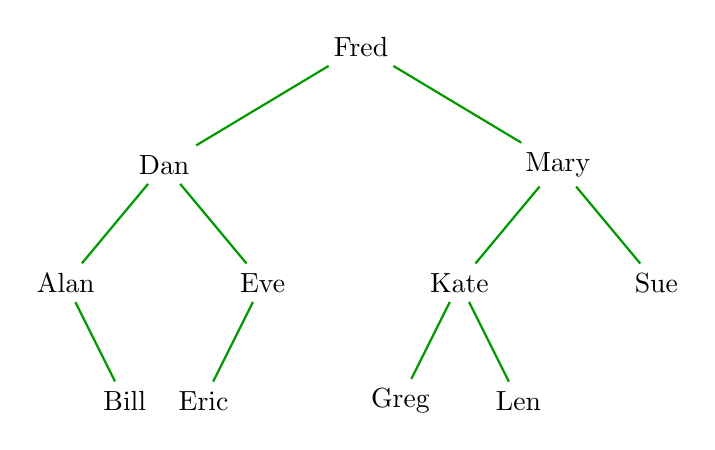
\begin{tikzpicture}[
    % Cấu hình khoảng cách
    level distance=1.5cm,               % Khoảng cách giữa các tầng
    level 1/.style={sibling distance=5cm}, % Khoảng cách nhánh tầng 1
    level 2/.style={sibling distance=2.5cm}, % Khoảng cách nhánh tầng 2
    level 3/.style={sibling distance=1.5cm}, % Khoảng cách nhánh tầng 3
    % Cấu hình đường nối (màu xanh, dày hơn chút)
    edge from parent/.style={draw, green!60!black, thick} 
]

% Bắt đầu vẽ từ Root
\node {Fred}
    % Nhánh Trái (Dan)
    child { node {Dan}
        % Con của Dan -> Alan (Trái)
        child { node {Alan}
            child[missing] { node {} } % Alan không có con trái -> missing
            child { node {Bill} }      % Con phải của Alan
        }
        % Con của Dan -> Eve (Phải)
        child { node {Eve}
            child { node {Eric} }      % Con trái của Eve
            child[missing] { node {} } % Eve không có con phải -> missing
        }
    }
    % Nhánh Phải (Mary)
    child { node {Mary}
        % Con của Mary -> Kate (Trái)
        child { node {Kate}
            child { node {Greg} }
            child { node {Len} }
        }
        % Con của Mary -> Sue (Phải)
        child { node {Sue} }
    };

\end{tikzpicture}
\\\small\textbf{\textit{Khóa là xâu ký tự}}
\end{center}
\end{column}
\end{columns}
\end{frame}

\begin{frame}{Biểu diễn cây nhị phân tìm kiếm}
    \centering
    % Dùng resizebox để hình tự co lại cho vừa chiều ngang slide (0.95 textwidth)
    \resizebox{0.95\textwidth}{!}{%
        \begin{tikzpicture}
            % --- ĐỊNH NGHĨA MÀU SẮC ---
            \definecolor{myblue}{RGB}{100, 149, 237}
            \definecolor{memblue}{RGB}{200, 230, 255}
            \definecolor{memcyan}{RGB}{0, 255, 255}
            \definecolor{memgreen}{RGB}{200, 255, 200}
        
            % --- PHẦN 1: CÂY LOGIC (BÊN TRÁI) ---
            % Dời sang trái 8cm để tách biệt với phần bộ nhớ
            \begin{scope}[local bounding box=logicaltree, xshift=-8cm, yshift=2cm]
                \tikzset{
                    treenode/.style={circle, draw=black, fill=myblue, text=white, minimum size=0.8cm, font=\bfseries},
                    level 1/.style={sibling distance=2.5cm},
                    level 2/.style={sibling distance=1.5cm},
                    edge from parent/.style={draw, thick, black}
                }
                
                \node[treenode] {7}
                    child { node[treenode] {2} }
                    child { node[treenode] {20}
                        child { node[treenode] {9} 
                            child[missing] {}
                            child { node[treenode] {11} }
                        }
                        child { node[treenode] {25} }
                    };
                % Label chú thích dưới cây logic
                \node[below=0.5cm of logicaltree] {\textbf{Cây Logic}};
            \end{scope}
        
            % --- PHẦN 2: CẤU TRÚC BỘ NHỚ (BÊN PHẢI) ---
            \begin{scope}[scale=0.7, transform shape, xshift=2cm, local bounding box=memorystruct]
            \tikzset{
                struct/.style={
                    rectangle split,
                    rectangle split parts=4,
                    rectangle split horizontal,
                    draw,
                    anchor=north,
                    rectangle split part fill={memblue, memcyan, memblue, memgreen},
                    minimum height=0.8cm
                },
                ptr/.style={->, >=stealth, thick},
                parentptr/.style={->, >=stealth, thick, dashed, magenta},
                ground/.style={shorten >=0pt}
            }
        
            % Các Node bộ nhớ (Giữ nguyên vị trí tương đối)
            \node[struct] (n7) at (0,3) { \nodepart{one}\it left \nodepart{two}\bf 7 \nodepart{three}\it right \nodepart{four} NIL };
            \node[struct] (n2) at (-3, 0.5) { \nodepart{one}\it left \nodepart{two}\bf 2 \nodepart{three}\it right \nodepart{four} $p$ };
            \node[struct] (n20) at (3, 0.5) { \nodepart{one}\it left \nodepart{two}\bf 20 \nodepart{three}\it right \nodepart{four} $p$ };
            \node[struct] (n9) at (0, -2.5) { \nodepart{one}\it left \nodepart{two}\bf 9 \nodepart{three}\it right \nodepart{four} $p$ };
            \node[struct] (n25) at (5, -2.5) { \nodepart{one}\it left \nodepart{two}\bf 25 \nodepart{three}\it right \nodepart{four} $p$ };
            \node[struct] (n11) at (2, -5) { \nodepart{one}\it left \nodepart{two}\bf 11 \nodepart{three}\it right \nodepart{four} $p$ };
        
            % Vẽ liên kết
            \draw[ptr] (n7.one south) -- (n2.north);
            \draw[ptr] (n7.three south) -- (n20.north);
            \draw[ptr] (n20.one south) -- (n9.north);
            \draw[ptr] (n20.three south) -- (n25.north);
            \draw[ptr] (n9.three south) -- (n11.north);
        
            % Liên kết Parent
            \draw[parentptr] (n2.four north) .. controls +(0.5,1) and +(-0.5,-1) .. (n7.two south);
            \draw[parentptr] (n20.four north) .. controls +(-0.5,1) and +(0.5,-1) .. (n7.three south);
            \draw[parentptr] (n9.four north) .. controls +(0.5,1) and +(-0.5,-1) .. (n20.two south);
            \draw[parentptr] (n25.four north) .. controls +(-0.5,1) and +(0.5,-1) .. (n20.three south);
            \draw[parentptr] (n11.four north) .. controls +(-0.5,1) and +(0.5,-1) .. (n9.three south);
        
            % Grounding
            \drawground{n2.one south} \drawground{n2.three south}
            \drawground{n9.one south}
            \node at ($(n9.one south) + (-0.5, -0.5)$) [text=gray, font=\scriptsize] {NULL};
            \drawground{n25.one south} \drawground{n25.three south}
            \drawground{n11.one south} \drawground{n11.three south}
        \end{scope}
            % Label chú thích dưới bộ nhớ
            \node[below=6cm of n7] {\textbf{Cấu trúc chi tiết}};
            
        \end{tikzpicture}
    } % Kết thúc resizebox
\end{frame}
\subsection{Tìm kiếm trên BST}
% --- Search BST ---
\begin{frame}[fragile]{3.1. Tìm kiếm trên BST}
    \begin{columns}
        \begin{column}{0.55\textwidth}
    \textbf{Ý tưởng:} So sánh $target$ với $key$ của nút hiện tại.
    \begin{itemize}
        \item Nhỏ hơn: Đi sang trái.
        \item Lớn hơn: Đi sang phải.
        \item Bằng: Tìm thấy.
    \end{itemize}
    
    
            \begin{minted}{c}
TreeNode* search(TreeNode* node, float target) {
    if (node != NULL) {
        if (target < node->key)
            return search(node->leftPtr, target);
        else if (target > node->key)
            return search(node->rightPtr, target);
    }
    return node; // Trả về node hoặc NULL
}
            \end{minted}
        \end{column}
        \begin{column}{0.4\textwidth}
            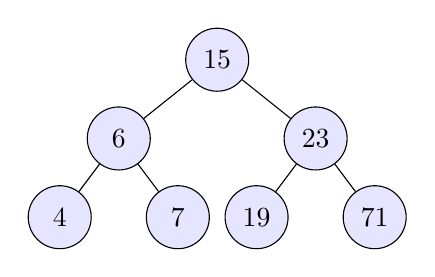
\begin{tikzpicture}[
        level distance=1cm,
        sibling distance=2.5cm,
        level 2/.style={sibling distance=1.5cm},
        nodes={treenode} 
    ]
        % --- QUAN TRỌNG: Đặt tên node gốc là (root) ---
        \node (root) {15} 
            child {node {6}
                child {node {4}}
                child {node {7}}
            }
            child {node {23}
                child {node {19}}
                child {node {71}}
            };
            
    \end{tikzpicture}
            \\\textbf{Độ phức tạp:} $O(h)$ \\($h$ là chiều cao cây).
        \end{column}
    \end{columns}
\end{frame}

\begin{frame}[t]{3.1. Tìm kiếm trên BST}
    \textbf{Ví dụ: Tìm kiếm giá trị $X = 7$}

    \begin{center}
        \begin{tikzpicture}[
            level distance=1.2cm,
            sibling distance=3.5cm,
            level 2/.style={sibling distance=1.8cm},
            % Style cho node thường
            treenode/.style={
                circle, draw=HUSTBlue, thick, fill=white, 
                minimum size=0.8cm, font=\bfseries
            },
            % Style cho node đang xét (Active)
            active/.style={
                circle, draw=HUSTRed, very thick, fill=HUSTRed!10, 
                minimum size=0.9cm, font=\bfseries\color{HUSTRed}
            },
            % Style cho node tìm thấy (Found)
            found/.style={
                circle, draw=green!60!black, very thick, fill=green!10, 
                minimum size=0.9cm, font=\bfseries\color{green!60!black}
            },
            % Style mũi tên tìm kiếm
            searchptr/.style={
                ->, >=stealth, HUSTRed, ultra thick, dashed, 
                shorten >=2pt, shorten <=2pt
            }
        ]

            % --- 1. VẼ CÂY ---
            \node[treenode] (root) {15}
                child {
                    node[treenode] (n6) {6}
                    child { node[treenode] (n4) {4} }
                    child { node[found] (n7) {7} } % Node tìm thấy
                }
                child {
                    node[treenode] (n23) {23}
                    child { node[treenode] (n19) {19} }
                    child { node[treenode] (n71) {71} }
                };

            % --- 2. VẼ ĐƯỜNG ĐI TÌM KIẾM ---
            % Từ 15 xuống 6
            \draw[searchptr, bend right=30] (root.west) to node[left, font=\scriptsize, color=HUSTRed] {$7 < 15$} (n6.north west);
            
            % Từ 6 xuống 7
            \draw[searchptr, bend left=30] (n6.east) to node[right, font=\scriptsize, color=HUSTRed] {$7 > 6$} (n7.north east);

            % --- 3. CHÚ THÍCH BÊN CẠNH ---
            \node[right=1cm of n23, text width=5cm, anchor= west, font=\small] {
                \textbf{Quy trình:}
                \begin{itemize}
                    \item[1.] So sánh $x=7$ với gốc \textbf{15}: \\
                    $7 < 15 \Rightarrow$ Đi sang trái.
                    \item[2.] So sánh $x=7$ với \textbf{6}: \\
                    $7 > 6 \Rightarrow$ Đi sang phải.
                    \item[3.] So sánh $x=7$ với \textbf{7}: \\
                    $7 == 7 \Rightarrow$ \textcolor{green!60!black}{\textbf{Tìm thấy!}}
                \end{itemize}
            };

        \end{tikzpicture}
    \end{center}
\end{frame}

\begin{frame}[fragile]{3.1. Tìm kiếm trên BST}
    \textbf{Ví dụ: Tìm kiếm giá trị $X = 9$}
    
    \vspace{0.5cm}
    \begin{columns}
        % --- CỘT TRÁI: HÌNH VẼ ---
        \begin{column}{0.55\textwidth}
            \centering
            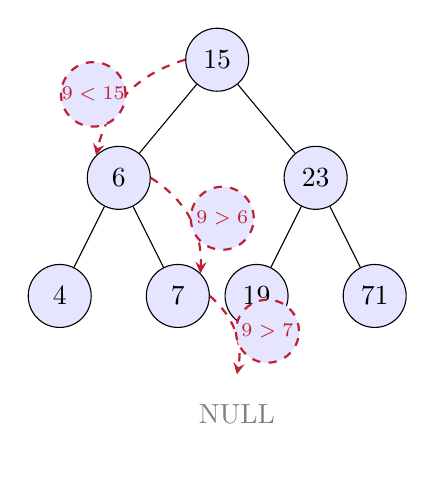
\begin{tikzpicture}[
                level distance=1.5cm,
                sibling distance=2.5cm,
                level 2/.style={sibling distance=1.5cm},
                nodes={treenode}, % Style node tròn xanh đã định nghĩa trước đó
                searchptr/.style={->, >=stealth, dashed, HUSTRed, thick, font=\scriptsize\bfseries}
            ]
                % 1. VẼ CÂY
                \node (root) {15}
                    child { node (n6) {6}
                        child { node (n4) {4} }
                        child { node (n7) {7} 
                            % Thêm node ảo (missing) bên trái và node NULL bên phải để minh hoạ
                            child[missing] 
                            child { node[draw=none, fill=none] (null) {\textcolor{gray}{NULL}} edge from parent[draw=none]} 
                        }
                    }
                    child { node (n23) {23}
                        child { node (n19) {19} }
                        child { node (n71) {71} }
                    };

                % 2. VẼ ĐƯỜNG ĐI TÌM KIẾM (Mũi tên đỏ nét đứt)
                
                % Bước 1: 9 < 15 -> Sang trái
                \draw[searchptr, bend right=30] (root.west) to node[left] {$9 < 15$} (n6.north west);
                
                % Bước 2: 9 > 6 -> Sang phải
                \draw[searchptr, bend left=30] (n6.east) to node[right] {$9 > 6$} (n7.north east);
                
                % Bước 3: 9 > 7 -> Sang phải (gặp NULL)
                \draw[searchptr, bend left=30] (n7.east) to node[right] {$9 > 7$} (null.north);

            \end{tikzpicture}
        \end{column}

        % --- CỘT PHẢI: GIẢI THÍCH ---
        \begin{column}{0.45\textwidth}
            \textbf{Quy trình:}
            \begin{enumerate}
                \item So sánh $x=9$ với gốc 15:
                \\ $9 < 15 \Rightarrow$ Đi sang trái.
                
                \item So sánh $x=9$ với 6:
                \\ $9 > 6 \Rightarrow$ Đi sang phải.
                
                \item So sánh $x=9$ với 7:
                \\ $9 > 7 \Rightarrow$ Đi sang phải.
                
                \item \textbf{Kết luận:}
                \\ Nhánh phải của 7 là \texttt{NULL}.
                \\ $\Rightarrow$ \textcolor{HUSTRed}{\textbf{Không tìm thấy!}}
            \end{enumerate}
        \end{column}
    \end{columns}
\end{frame}

% --- Min/Max BST ---
\subsection{Tìm Min/Max}
\begin{frame}[fragile]{3.2. Tìm Min / Max}
    \begin{columns}
        \begin{column}{0.48\textwidth}
            \textbf{Tìm Min:} Đi về phía bên trái cùng.
            \begin{minted}{c}
TreeNode* find_min(TreeNode* T) {
    if (T == NULL) return NULL;
    else if (T->leftPtr == NULL) 
        return T;
    else 
        return find_min(T->leftPtr);
}
            \end{minted}
            \textbf{Tìm Max:} Đi về phía bên phải cùng.
            \begin{minted}{c}
TreeNode* find_max(TreeNode* T) {
    if (T != NULL)
        while (T->rightPtr != NULL)
            T = T->rightPtr;
    return T;
}
            \end{minted}
        \end{column}
        \begin{column}{0.48\textwidth}
            \centering
            \vspace{0.5cm} % Đẩy hình xuống xíu cho cân
            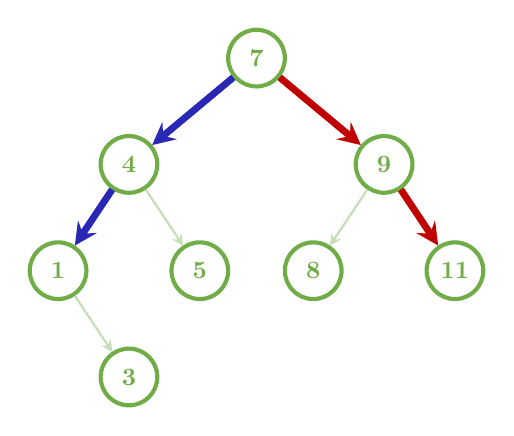
\begin{tikzpicture}[
                scale=0.9, transform shape,
                % Style cho các Node
                bstnode/.style={
                    circle, 
                    draw=bstgreen, line width=1.5pt,
                    fill=white, 
                    text=bstgreen, font=\bfseries, 
                    minimum size=0.8cm, inner sep=0pt
                },
                % Style cho đường nối thường
                normedge/.style={
                    ->, >=stealth, thick, color=bstgreen!40
                },
                % Style cho đường tìm MIN (Xanh đậm)
                minpath/.style={
                    ->, >=stealth, line width=2.5pt, color=pathblue
                },
                % Style cho đường tìm MAX (Đỏ đậm)
                maxpath/.style={
                    ->, >=stealth, line width=2.5pt, color=pathred
                }
            ]
                % 1. Vẽ các Node (Tọa độ thủ công cho giống hình)
                \node[bstnode] (n7) at (0,0) {7};
                \node[bstnode] (n4) at (-1.8,-1.5) {4};
                \node[bstnode] (n9) at (1.8,-1.5) {9};
                
                \node[bstnode] (n1) at (-2.8,-3.0) {1};
                \node[bstnode] (n5) at (-0.8,-3.0) {5};
                \node[bstnode] (n8) at (0.8,-3.0) {8};
                \node[bstnode] (n11) at (2.8,-3.0) {11};
                
                \node[bstnode] (n3) at (-1.8,-4.5) {3};

                % 2. Vẽ các đường nối thường (mờ)
                \draw[normedge] (n4) -- (n5);
                \draw[normedge] (n1) -- (n3);
                \draw[normedge] (n9) -- (n8);

                % 3. Vẽ đường tìm Min (Xanh đậm - Đi trái hết)
                \draw[minpath] (n7) -- (n4);
                \draw[minpath] (n4) -- (n1);

                % 4. Vẽ đường tìm Max (Đỏ đậm - Đi phải hết)
                \draw[maxpath] (n7) -- (n9);
                \draw[maxpath] (n9) -- (n11);

            \end{tikzpicture}
        \end{column}
    \end{columns}
\end{frame}
\subsection{Kế cận trước và Kế cận sau}
\begin{frame}[t]{3.3. Kế cận trước và Kế cận sau}
    \color{HUSTBlue}
    \begin{itemize}
    \item \textbf{Kế cận sau} (Successor) của nút $x$ là nút $y$ sao cho $key[y]$ là khoá nhỏ nhất còn lớn hơn $key[x]$.
    \begin{itemize}
        \item Kế cận sau của nút với khoá lớn nhất là NULL.
    \end{itemize}
    \item \textbf{Kế cận trước} (Predcessor) của nút $x$ là nút $y$ sao cho $key[y]$ là khoá lớn nhất còn nhỏ hơn $key[x]$.
    \begin{itemize}
    \item Kế cận trước của nút với khoá nhỏ nhất là NULL.
    \end{itemize}
    \item Việc tìm kiếm kế cận sau/trước được thực hiện mà không cần thực hiện so sánh khoá.
\end{itemize}
\end{frame}
\begin{frame}[t]{3.3. Kế cận trước và Kế cận sau}
    \vspace{-0.5em}
    {\large
    10, 20, \textcolor{textred}{23}, 25, 30, 31, 35, \textcolor{textpink}{37}, \textcolor{textred}{50}, \textcolor{textorange}{53}, 55, 60, 62
    }
    
    \vspace{0.3cm}
    
    \centering
    \resizebox{0.95\textwidth}{!}{% <--- Quan trọng: % để không bị lỗi khoảng trắng
    \begin{tikzpicture}[
        % --- CẤU HÌNH KHOẢNG CÁCH CÂY ---
        level 1/.style={sibling distance=7cm, level distance=1.5cm},
        level 2/.style={sibling distance=3.5cm, level distance=1.5cm},
        level 3/.style={sibling distance=2cm, level distance=1.5cm},
        level 4/.style={sibling distance=1.5cm, level distance=1.5cm},
        % --- STYLE ---
        treenode/.style={
            circle, draw=black!50, fill=nodeblue, text=white, 
            font=\bfseries, minimum size=1cm, inner sep=0pt
        },
        patharrow/.style={
            ->, >=stealth, red, line width=1.5pt
        },
        yellowarrow/.style={
            single arrow, draw=black, fill=yellow, 
            minimum height=0.8cm, minimum width=0.5cm, 
            single arrow head extend=0.1cm, anchor=tip
        }
    ]
        % --- 1. VẼ CÂY ---
        \node[treenode, text=textred] (n50) {50}
            child { node[treenode] (n30) {30}
                child { node[treenode] (n25) {25}
                    child { node[treenode] (n10) {10} 
                        child[missing] 
                        child { node[treenode] (n20) {20} 
                            child[missing] 
                            child { node[treenode, text=textred] (n23) {23} }
                        }
                    }
                    child[missing] 
                }
                child { node[treenode] (n35) {35}
                    child { node[treenode] (n31) {31} }
                    child { node[treenode, text=textpink] (n37) {37} }
                }
            }
            child { node[treenode] (n55) {55}
                child[sibling distance=2.5cm] { node[treenode, text=textorange] (n53) {53} }
                child[sibling distance=2.5cm] { node[treenode] (n60) {60} 
                    child[missing] 
                    child { node[treenode] (n62) {62} }
                }
            };

        % --- 2. NHÃN X VÀ Y ---
        \node[left=0.8cm of n50, font=\bfseries\large] (lblx) {x};
        \node[yellowarrow, rotate=0] at ($(n50.west)+(0.1,0)$) {};
        
        \node[left=0.8cm of n23, font=\bfseries\large] (lbly) {y};
        \node[yellowarrow, rotate=0] at ($(n23.west)+(0.1,0)$) {};

        % --- 3. MŨI TÊN ĐỎ (ĐƯỜNG ĐI) ---
        \draw[patharrow, bend left=35] (n50.south east) to (n53.north);
        \draw[patharrow, bend right=35] (n50.south west) to (n37.north);
        \draw[patharrow, bend left=40] (n23.north west) to (n20.south west);
        \draw[patharrow, bend left=40] (n20.north west) to (n10.south west);
        \draw[patharrow, bend left=40] (n10.north) to (n25.south west);

        % --- 4. CÁC TEXT CHÚ THÍCH ---
        \node[below right=0.8cm and -0.2cm of n53, align=left, text width=4.5cm, font=\small] {
            \textcolor{textorange}{\textbf{Successor}} của \textbf{x} \\
            là nút trái nhất \\
            trong cây con phải của nó
        };
        \node[yellowarrow, rotate=120] at ($(n53.south east)+(0.2,-0.1)$) {};

        \node[below=1.2cm of n37, align=center, text width=5cm, font=\small] {
            \textcolor{textpink}{\textbf{Predecessor}} của \textbf{x} \\
            là nút phải nhất trong \\
            cây con trái của nó
        };
        \node[yellowarrow, rotate=90] at ($(n37.south)+(0,-0.2)$) {};

        \node[above left=1cm and 0.2cm of n25, align=right, text width=5.5cm, font=\small] {
            \textcolor{textorange}{\textbf{Successor}} của \textbf{y} là tổ tiên \\
            gần nhất có con trái hoặc là \\
            \textbf{y} hoặc là tổ tiên của \textbf{y}
        };
        \node[yellowarrow, rotate=-45] at ($(n25.north west)+(-0.1,0.1)$) {};

        \node[left=0cm of n10, align=left, text width=4.5cm, font=\small] {
            \textcolor{textorange}{\textbf{Predessor}} của \textbf{y} là tổ tiên \\
            gần nhất có con phải \\
            hoặc là \textbf{y} hoặc là tổ tiên \\
            của \textbf{y}
        };
        \node[yellowarrow, rotate=-20] at ($(n20.north west)+(-1,0)$) {};
        
        \node[left=1.5cm of n23, align=right, text width=3.5cm, anchor=east, font=\small] {
            \textbf{y} không có cây con \\
            cả trái lẫn phải
        };

    \end{tikzpicture}% <--- Quan trọng: % ở đây
    }
\end{frame}
\begin{frame}[t]{3.3. Kế cận trước và Kế cận sau}
    \textbf{\large Tìm kế cận sau (2 tình huống)}\\
    a. Nếu \textbf{$x$ có con phải} thì kế cận sau của $x$ sẽ là nút $y$ với khoá $key[y]$ nhỏ\\
    ($y$ là nút trái nhất trong cây con phải của $x$).\\
    \begin{itemize}
        \item Để tìm y có thể dùng find-min(x$\to$rightPtr):
        \begin{center}
        \textbf{$y=$ find-min(x$\to$rightPtr)}
        \end{center}
        \item hoặc bắt đầu từ gốc của cây con phải luôn đi theo con trái đến khi gặp nút không có con trái $\to$ nút y cần tìm.
    \end{itemize}
\end{frame}
\begin{frame}[t]{3.3. Kế cận trước và Kế cận sau}
    \textbf{\large Tìm kế cận sau (2 tình huống)}\\
    b. Nếu $x$ không có con phải thì kế cận sau của $x$ là tổ tiên gần nhất có con trái hoặc là $x$ hoặc là tổ tiên của $x$. Tìm kế cận sau:\\
    \begin{itemize}
        \item Bắt đầu từ $x$ cần di chuyển lên trên (theo con trỏ parent) cho đến khi gặp nút $y$ có con trái đầu tiên thì dừng: $y$ là kế cận sau của $x$.
        \item Nếu không thể di chuyển tiếp được lên trên (tức là đã đến gốc) thì x là nút lớn nhất(và vì thế x không có kế cận sau).
    \end{itemize}
\end{frame}
\begin{frame}[t]{3.3. Kế cận trước và Kế cận sau}
    \textbf{\large Tìm kế cận trước (2 tình huống)}\\
    a. Nếu x có con trái thì kế cận trước của x sẽ là nút y với khoá key[y] lớn nhất trong cây con
trái của x\\
    \begin{itemize}
        \item (y là nút phải nhất nhất trong cây con trái của x):
    \end{itemize}
            \begin{center}
    \textbf{$y = \text{find\_max}(x \to \text{leftPtr})$} 
\end{center}
    b. Nếu x không có con trái thì kế cận trước của x là tổ tiên gần nhất có con phải hoặc là x
hoặc là tổ tiên của x.
\end{frame}
% --- Insert BST ---
\subsection{Bổ sung 1 nút vào BST}
\begin{frame}[t]{3.4. Bổ sung 1 nút vào BST}
    
    \vspace{0.2cm}
    \textbf{\large \textcolor{textdark}{Ví dụ 1:} Bổ sung $z = 32$}
    \vspace{0.2cm}

    \centering
    \resizebox{0.95\textwidth}{!}{%
    \begin{tikzpicture}[
        % --- CẤU HÌNH CHUNG ---
        level distance=1.2cm,
        sibling distance=1.5cm,
        % Style cho Node
        treenode/.style={
            circle, 
            draw=black!80, 
            fill=nodeblue, 
            text=white, 
            font=\bfseries, 
            minimum size=0.8cm, 
            inner sep=0pt,
            thick
        },
        % Style cho cạnh
        edge from parent/.style={draw, thick, black},
        % Style cho mũi tên vàng chuyển bước
        steparrow/.style={
            single arrow, draw=black!50, fill=yellow!30, 
            minimum height=1.5cm, minimum width=0.5cm, 
            single arrow head extend=0.1cm, anchor=tail
        }
    ]

        % ==========================================
        % BƯỚC 1: CÂY TRÊN CÙNG (GỐC)
        % ==========================================
        \node[treenode] (root1) at (0,0) {25}
            child { node[treenode] {20} 
                child { node[treenode] {12} }
                child[missing]
            }
            child { node[treenode] {35} 
                child[missing]
                child { node[treenode] {40} }
            };
        
        % Nhãn x
        \node[above left=0.1cm of root1, gray] {$x$};
        
        % Text giải thích bước 1 (Bên phải)
        \node[right=0.5cm of root1, align=left, text width=5cm, text=textdark] {
            So sánh 32 và 25 \\
            duyệt tiếp cây con phải
        };

        % ==========================================
        % BƯỚC 2: CÂY BÊN TRÁI (DUYỆT XUỐNG)
        % ==========================================
        \node[treenode] (root2) at (-4,-4.5) {25}
            child { node[treenode] {20} 
                child { node[treenode] {12} }
                child[missing]
            }
            child { node[treenode] (node35_2) {35} 
                child[missing]
                child { node[treenode] {40} }
            };
            
        % Vẽ ký hiệu NULL (đất) cho con trái của 35
        \draw[thick] (node35_2) -- ++(-0.6,-0.8) coordinate (ground);
        \draw[thick] ($(ground)+(-0.2,0)$) -- ($(ground)+(0.2,0)$);
        
        % Nhãn x, y
        \node[above left=0.1cm of root2, gray] {$x$};
        \node[above right=0.1cm of node35_2, gray] {$y$};

        % Text giải thích bước 2 (Bên trái)
        \node[left=0.5cm of root2, align=left, text width=4cm, text=textdark] {
            So sánh 32 và 35, \\
            duyệt tiếp \\
            cây con trái
        };

        % ==========================================
        % BƯỚC 3: CÂY BÊN PHẢI (KẾT QUẢ)
        % ==========================================
        \node[treenode] (root3) at (4,-4.5) {25}
            child { node[treenode] {20} 
                child { node[treenode] {12} }
                child[missing]
            }
            child { node[treenode] (node35_3) {35} 
                child { node[treenode] (node32) {32} }
                child { node[treenode] {40} }
            };
            
        % Nhãn y, z
        \node[above right=0.1cm of node35_3, gray] {$y$};
        \node[right=0.1cm of node32, gray] {$z$};

        % Text giải thích bước 3 (Bên phải)
        \node[right=0.1cm of node35_3, align=left, anchor=west, text=textdark] {
            chèn 32 như là con trái
        };

        % ==========================================
        % MŨI TÊN CHUYỂN BƯỚC (VÀNG)
        % ==========================================
        
        % Mũi tên 1: Từ trên xuống trái (Đã chỉnh lại vị trí và góc xoay)
        \node[steparrow, rotate=-135] at (-2.5,-2.5) {};
        
        % Mũi tên 2: Từ trái sang phải (Đã chỉnh lại vị trí)
        \node[steparrow, rotate=0] at (-0.5,-5) {};

    \end{tikzpicture}
    }
\end{frame}

\begin{frame}[fragile]{3.4. Bổ sung nút vào BST}
    \textbf{Quy tắc:}
    \begin{itemize}
        \item Nếu cây rỗng, tạo nút mới là gốc.
        \item Nếu $x < key$, chèn vào cây con trái.
        \item Nếu $x > key$, chèn vào cây con phải.
    \end{itemize}

    \begin{columns}
        \begin{column}{0.6\textwidth}
            \begin{minted}{c}
TreeNode* insert(TreeNode* node, float item) {
    if (node == NULL) {
        node = makeTreeNode(item); // Tạo nút mới
    } else if (item < node->key) {
        node->leftPtr = insert(node->leftPtr, item);
    } else if (item > node->key) {
        node->rightPtr = insert(node->rightPtr, item);
    }
    return node;
}
            \end{minted}
        \end{column}
        \begin{column}{0.35\textwidth}
            \centering
            Thời gian tính: O(h),\\
h là độ cao của BST
        \end{column}
    \end{columns}
\end{frame}
\begin{frame}[t]{3.4. Bổ sung 1 nút vào BST}
    
    \vspace{0.2cm}
    
    \begin{columns}[T]
        % --- CỘT TRÁI: VÍ DỤ VÀ NODE CẦN THÊM ---
        \begin{column}{0.25\textwidth}
            \vspace{0.5cm}
            \textbf{\large \textcolor{textdark}{Ví dụ 2}}
            
            \vspace{1cm}
            \centering
            % Node cần thêm (57)
            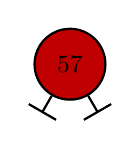
\begin{tikzpicture}
                \node[circle, draw=black, thick, fill=nodered, text=black, font=\small, minimum size=0.9cm] (n57) {57};
                
                % Vẽ 2 chân NULL cho node 57 (Vẽ thủ công vì lệnh drawleaf ở ngoài có thể chưa nhận trong scope nhỏ này nếu không truyền đúng)
                \draw[thick] (n57) -- ++(-120:0.7) coordinate (l);
                \draw[thick] ($(l)+(-30:0.2)$) -- ($(l)+(150:0.2)$);
                \draw[thick] (n57) -- ++(-60:0.7) coordinate (r);
                \draw[thick] ($(r)+(-150:0.2)$) -- ($(r)+(30:0.2)$);
            \end{tikzpicture}
        \end{column}
        
        % --- CỘT PHẢI: CÂY BST ---
        \begin{column}{0.75\textwidth}
            \centering
            % Dùng scale thay vì resizebox để an toàn
            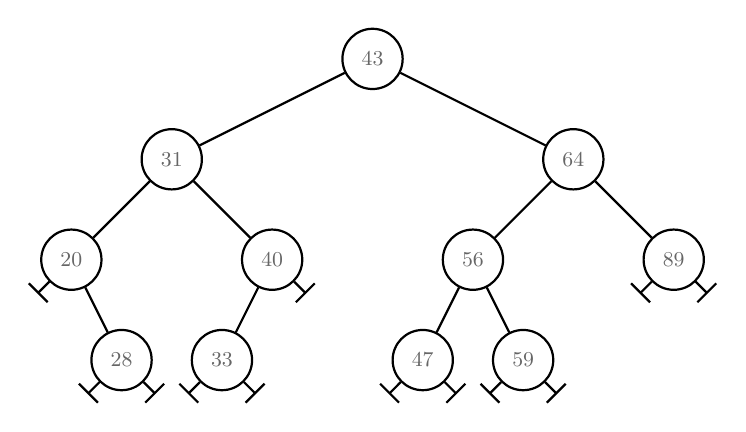
\begin{tikzpicture}[
                scale=0.85, transform shape,
                level distance=1.5cm,
                level 1/.style={sibling distance=6cm},
                level 2/.style={sibling distance=3cm},
                level 3/.style={sibling distance=1.5cm},
                treenode/.style={
                    circle, draw=black, thick, fill=white, 
                    text=black!60, font=\small, minimum size=0.9cm, inner sep=0pt
                },
                edge from parent/.style={draw, thick, black}
            ]

                % --- VẼ CÂY ---
                \node[treenode] (n43) {43}
                    child { node[treenode] (n31) {31}
                        child { node[treenode] (n20) {20} 
                            child[missing] 
                            child { node[treenode] (n28) {28} }
                        }
                        child { node[treenode] (n40) {40}
                            child { node[treenode] (n33) {33} }
                            child[missing]
                        }
                    }
                    child { node[treenode] (n64) {64}
                        child { node[treenode] (n56) {56}
                            child { node[treenode] (n47) {47} }
                            child { node[treenode] (n59) {59} }
                        }
                        child { node[treenode] (n89) {89} }
                    };

                % --- VẼ CÁC CHÂN NULL (Dùng lệnh đã định nghĩa ở Preamble) ---
                \drawleaf{n20}{-135}
                \drawleaf{n28}{-135} \drawleaf{n28}{-45}
                \drawleaf{n40}{-45}
                \drawleaf{n33}{-135} \drawleaf{n33}{-45}
                \drawleaf{n47}{-135} \drawleaf{n47}{-45}
                \drawleaf{n59}{-135} \drawleaf{n59}{-45}
                \drawleaf{n89}{-135} \drawleaf{n89}{-45}

            \end{tikzpicture}
        \end{column}
    \end{columns}
\end{frame}
\begin{frame}[t]{3.4. Bổ sung 1 nút vào BST}
    
    \vspace{0.2cm}
    
    \begin{columns}[T]
        % --- CỘT TRÁI: TIÊU ĐỀ VÀ NODE MẪU ---
        \begin{column}{0.25\textwidth}
            \vspace{0.5cm}
            \textbf{\large \textcolor{textdark}{Ví dụ 2}}
            
            \vspace{1cm}
            \centering
            % Node 57 mẫu
            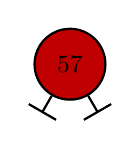
\begin{tikzpicture}
                \node[circle, draw=black, thick, fill=nodered, text=black, font=\small, minimum size=0.9cm] (n57sample) {57};
                \drawleaf{n57sample}{-120}
                \drawleaf{n57sample}{-60}
            \end{tikzpicture}
        \end{column}
        
        % --- CỘT PHẢI: CÂY BST VỚI ĐƯỜNG ĐI ---
        \begin{column}{0.75\textwidth}
            \centering
            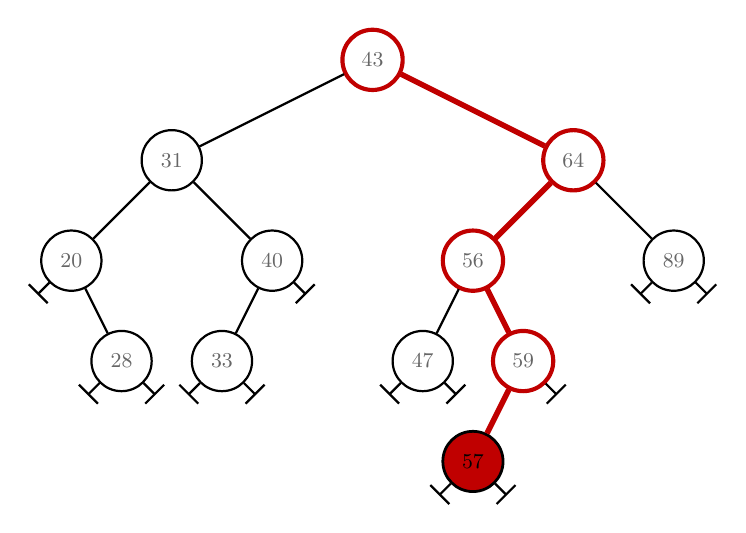
\begin{tikzpicture}[
                scale=0.85, transform shape,
                % Cấu hình khoảng cách
                level distance=1.5cm,
                level 1/.style={sibling distance=6cm},
                level 2/.style={sibling distance=3cm},
                level 3/.style={sibling distance=1.5cm},
                % --- CÁC STYLE ---
                % Node thường (Trắng, viền đen)
                treenode/.style={
                    circle, draw=black, thick, fill=white, 
                    text=black!60, font=\small, minimum size=0.9cm, inner sep=0pt
                },
                % Node trên đường đi (Trắng, viền ĐỎ dày)
                pathnode/.style={
                    treenode, draw=pathred, line width=1.5pt, text=black!60
                },
                % Node mới chèn (Nền ĐỎ, chữ đen)
                newnode/.style={
                    treenode, fill=nodered, text=black, draw=black, line width=1pt
                },
                % Cạnh thường
                edge from parent/.style={draw, thick, black},
                % Cạnh trên đường đi (Đỏ dày)
                pathedge/.style={draw, pathred, line width=2pt}
            ]

                % --- VẼ CÂY ---
                % Gốc 43 (Trên đường đi -> pathnode)
                \node[pathnode] (n43) {43}
                    % Nhánh Trái (Không đổi)
                    child { node[treenode] (n31) {31}
                        child { node[treenode] (n20) {20} 
                            child[missing] 
                            child { node[treenode] (n28) {28} }
                        }
                        child { node[treenode] (n40) {40}
                            child { node[treenode] (n33) {33} }
                            child[missing]
                        }
                    }
                    % Nhánh Phải (Đường đi chèn 57)
                    % Cạnh nối 43 -> 64 là màu đỏ (pathedge)
                    child[edge from parent/.style={pathedge}] { node[pathnode] (n64) {64}
                        % 64 -> 56 (Màu đỏ)
                        child[edge from parent/.style={pathedge}] { node[pathnode] (n56) {56}
                            % 56 -> 47 (Thường)
                            child[edge from parent/.style={draw, thick, black}] { node[treenode] (n47) {47} }
                            % 56 -> 59 (Màu đỏ)
                            child[edge from parent/.style={pathedge}] { node[pathnode] (n59) {59}
                                % 59 -> 57 (Màu đỏ - Node Mới)
                                child[edge from parent/.style={pathedge}] { node[newnode] (n57) {57} }
                                child[missing] % 59 không có phải
                            }
                        }
                        % 64 -> 89 (Thường)
                        child[edge from parent/.style={draw, thick, black}] { node[treenode] (n89) {89} }
                    };

                % --- VẼ CÁC CHÂN NULL (GROUND) ---
                % 1. Các node cũ
                \drawleaf{n20}{-135}
                \drawleaf{n28}{-135} \drawleaf{n28}{-45}
                \drawleaf{n40}{-45}
                \drawleaf{n33}{-135} \drawleaf{n33}{-45}
                \drawleaf{n47}{-135} \drawleaf{n47}{-45}
                \drawleaf{n89}{-135} \drawleaf{n89}{-45}
                
                % 2. Node 59 (Giờ đã có con trái là 57, chỉ còn thiếu con phải)
                \drawleaf{n59}{-45}
                
                % 3. Node mới 57 (Thiếu cả 2)
                \drawleaf{n57}{-135} \drawleaf{n57}{-45}

            \end{tikzpicture}
        \end{column}
    \end{columns}
\end{frame}
% --- Delete BST ---
\subsection{Loại bỏ nút trên BST}
\begin{frame}[fragile]{3.5. Loại bỏ nút trên BST}
    \textbf{Các tình huống:}
    \begin{enumerate}
        \item \textbf{Nút lá:} Xóa trực tiếp.
        \item \textbf{Có 1 con (Trái/Phải):} Nối cha của nút cần xóa với con duy nhất của nó.
        \item \textbf{Có 2 con:} 
            \begin{itemize}
                \item Tìm nút thế chỗ (thường là Min của cây con phải).
                \item Copy giá trị nút thế chỗ vào nút cần xóa.
                \item Xóa nút thế chỗ (quy về trường hợp 1 hoặc 2).
            \end{itemize}
    \end{enumerate}
    
    \vspace{0.2cm}
    \begin{columns}
        \begin{column}{0.5\textwidth}
            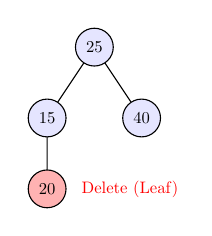
\begin{tikzpicture}[scale=0.6, transform shape, level/.style={sibling distance=20mm/#1}]
                \node[treenode] {25}
                    child { node[treenode] {15} 
                        child { node[treenode, fill=red!30] (del) {20} }
                    }
                    child { node[treenode] {40} };
                \node[right=0.2cm of del, red] {Delete (Leaf)};
            \end{tikzpicture}
        \end{column}
        \begin{column}{0.5\textwidth}
            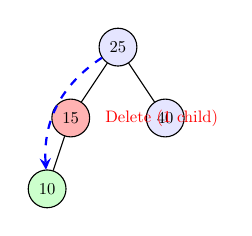
\begin{tikzpicture}[scale=0.6, transform shape, level/.style={sibling distance=20mm/#1}]
                \node[treenode] (root) {25}
                    child { node[treenode, fill=red!30] (del) {15} 
                        child { node[treenode, fill=green!20] {10} }
                        child[missing]
                    }
                    child { node[treenode] {40} };
                \draw[ptr, dashed, blue] (root) to [bend right] (del-1);
                \node[right=0.2cm of del, red] {Delete (1 child)};
            \end{tikzpicture}
        \end{column}
    \end{columns}
\end{frame}

\begin{frame}[t]{3.5. Loại bỏ 1 nút trên BST}
    \vspace{0.2cm}
    
    % --- KHUNG TEXT ---
    \begin{tikzpicture}
        \node[draw=black!50, align=left, text width=0.9\textwidth, inner sep=10pt] (box) {
            \textbf{\textcolor{textpurple}{Tình huống 1:}} \quad Nút cần xoá $x$ là lá (leaf) \\[0.5em]
            \textbf{\textcolor{gray}{Thao tác:}} \qquad \quad \quad Chữa lại nút cha của $x$ có con rỗng.
        };
    \end{tikzpicture}
    
    \vspace{0.5cm}
    \centering
    
    % --- CÂY BST ---
    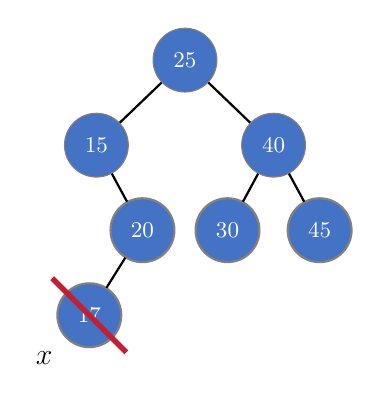
\begin{tikzpicture}[
        scale=0.9, transform shape,
        level distance=1.2cm,
        sibling distance=2.5cm,
        level 2/.style={sibling distance=1.3cm},
        level 3/.style={sibling distance=1.5cm},
        treenode/.style={
            circle, 
            draw=black!50, 
            fill=nodeblue, 
            text=white, 
            font=\small, 
            minimum size=0.9cm, 
            inner sep=0pt
        },
        edge from parent/.style={draw, thick, black}
    ]

        % Vẽ cây
        \node[treenode] (n25) {25}
            child { node[treenode] (n15) {15}
                child[missing] % 15 không có trái
                child { node[treenode] (n20) {20}
                    child { node[treenode] (n17) {17} } % Nút cần xoá
                    child[missing] % 20 không có phải
                }
            }
            child { node[treenode] (n40) {40}
                child { node[treenode] (n30) {30} }
                child { node[treenode] (n45) {45} }
            };

        % Ký hiệu nhãn x
        \node[below left=0.1cm of n17, font=\bfseries\large] {$x$};
        
        % VẼ DẤU GẠCH CHÉO ĐỎ TRÊN NÚT 17
        % Lấy toạ độ các góc của node 17 để gạch chéo
        \draw[HUSTRed, line width=2pt] ($(n17.north west)+(-0.2,0.2)$) -- ($(n17.south east)+(0.2,-0.2)$);
        % \draw[HUSTRed, line width=2pt] ($(n17.north east)+(0.2,0.2)$) -- ($(n17.south west)+(-0.2,-0.2)$); % Nếu muốn gạch chéo 2 đường (chữ X) thì bỏ comment dòng này

    \end{tikzpicture}
    
\end{frame}
\begin{frame}[t]{3.5. Loại bỏ 1 nút trên BST}
    \vspace{0.2cm}
    
    % --- 1. KHUNG TEXT MÔ TẢ ---
    \begin{tikzpicture}
        \node[draw=black!50, align=left, text width=0.92\textwidth, inner sep=8pt] (box) {
            \textbf{\textcolor{textpurple}{Tình huống 2:}} \quad Nút cần xoá $x$ có con trái mà không có con phải \\[0.5em]
            \textbf{\textcolor{black!70}{Thao tác:}} \qquad \quad \quad Gắn cây con trái của $x$ vào cha
        };
    \end{tikzpicture}
    
    \vspace{0.3cm}
    \centering
    
    % --- 2. HÌNH VẼ MINH HOẠ ---
    \resizebox{0.9\textwidth}{!}{%
    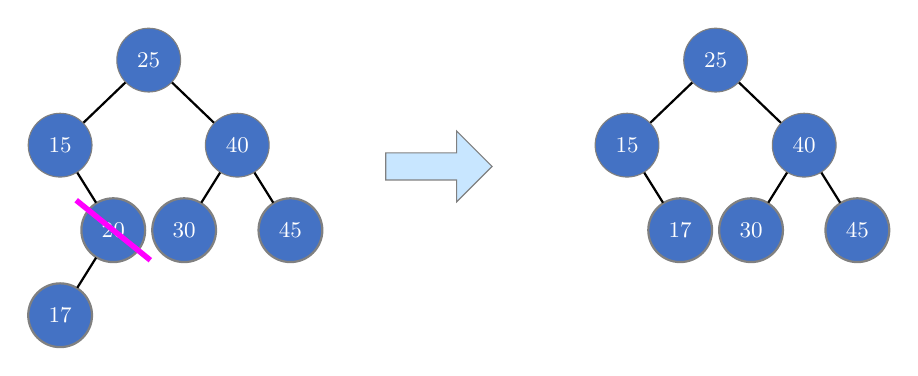
\begin{tikzpicture}[
        scale=0.9, transform shape,
        % Cấu hình chung
        level distance=1.2cm,
        sibling distance=2.5cm,
        level 2/.style={sibling distance=1.5cm},
        level 3/.style={sibling distance=1.5cm},
        % Style cho Node
        treenode/.style={
            circle, draw=black!50, fill=nodeblue, text=white, 
            font=\small, minimum size=0.9cm, inner sep=0pt
        },
        edge from parent/.style={draw, thick, black}
    ]

        % ======================================
        % CÂY BÊN TRÁI (TRƯỚC KHI XÓA)
        % ======================================
        \node[treenode] (root1) at (0,0) {25}
            child { node[treenode] {15}
                child[missing] % 15 không có trái
                child { node[treenode] (n20) {20} % NÚT CẦN XÓA
                    child { node[treenode] {17} } % Con trái của 20
                    child[missing] % 20 không có phải (Đúng tình huống 2)
                }
            }
            child { node[treenode] {40}
                child { node[treenode] {30} }
                child { node[treenode] {45} }
            };

        % Gạch chéo màu hồng trên node 20
        \draw[slashpink, line width=2pt] ($(n20.north west)+(-0.2,0.1)$) -- ($(n20.south east)+(0.2,-0.1)$);
        
        % ======================================
        % MŨI TÊN CHUYỂN ĐỔI (Ở GIỮA)
        % ======================================
        \node[single arrow, draw=black!50, fill=arrowblue, minimum height=1.5cm, minimum width=1cm, 
              single arrow head extend=0.2cm, anchor=center] at (4, -1.5) {};

        % ======================================
        % CÂY BÊN PHẢI (SAU KHI XÓA)
        % ======================================
        \begin{scope}[xshift=8cm]
            \node[treenode] (root2) at (0,0) {25}
                child { node[treenode] {15}
                    child[missing]
                    child { node[treenode] {17} } % 17 được gắn lên cha (15)
                }
                child { node[treenode] {40}
                    child { node[treenode] {30} }
                    child { node[treenode] {45} }
                };
        \end{scope}

    \end{tikzpicture}%
    }
\end{frame}
\begin{frame}[t]{3.5. Loại bỏ 1 nút trên BST}
    \vspace{0.2cm}
    
    % --- 1. KHUNG TEXT MÔ TẢ ---
    \begin{tikzpicture}
        \node[draw=black!50, align=left, text width=0.92\textwidth, inner sep=8pt] (box) {
            \textbf{\textcolor{textpurple}{Tình huống 3:}} \quad Nút cần xoá $x$ có con phải mà không có con trái \\[0.5em]
            \textbf{\textcolor{black!70}{Thao tác:}} \qquad \quad \quad Gắn cây con phải của $x$ vào cha
        };
    \end{tikzpicture}
    
    \vspace{0.3cm}
    \centering
    
    % --- 2. HÌNH VẼ MINH HOẠ ---
    \resizebox{0.9\textwidth}{!}{%
    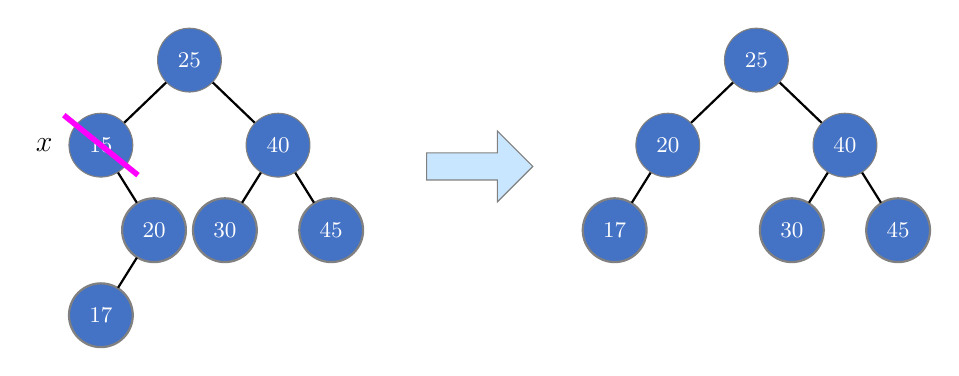
\begin{tikzpicture}[
        scale=0.9, transform shape,
        % Cấu hình chung
        level distance=1.2cm,
        sibling distance=2.5cm,
        level 2/.style={sibling distance=1.5cm},
        level 3/.style={sibling distance=1.5cm},
        % Style cho Node
        treenode/.style={
            circle, draw=black!50, fill=nodeblue, text=white, 
            font=\small, minimum size=0.9cm, inner sep=0pt
        },
        edge from parent/.style={draw, thick, black}
    ]

        % ======================================
        % CÂY BÊN TRÁI (TRƯỚC KHI XÓA)
        % ======================================
        \node[treenode] (root1) at (0,0) {25}
            child { node[treenode] (n15) {15} % NÚT CẦN XÓA (x)
                child[missing] % 15 không có trái (Đúng tình huống 3)
                child { node[treenode] {20} % Con phải của 15
                    child { node[treenode] {17} } 
                    child[missing] 
                } 
            }
            child { node[treenode] {40}
                child { node[treenode] {30} }
                child { node[treenode] {45} }
            };

        % Nhãn x
        \node[left=0.1cm of n15, font=\bfseries\large] {$x$};

        % Gạch chéo màu hồng trên node 15
        \draw[slashpink, line width=2pt] ($(n15.north west)+(-0.2,0.1)$) -- ($(n15.south east)+(0.2,-0.1)$);
        
        % ======================================
        % MŨI TÊN CHUYỂN ĐỔI (Ở GIỮA)
        % ======================================
        \node[single arrow, draw=black!50, fill=arrowblue, minimum height=1.5cm, minimum width=1cm, 
              single arrow head extend=0.2cm, anchor=center] at (4, -1.5) {};

        % ======================================
        % CÂY BÊN PHẢI (SAU KHI XÓA)
        % ======================================
        \begin{scope}[xshift=8cm]
            \node[treenode] (root2) at (0,0) {25}
                child { node[treenode] {20} % 20 được gắn lên thay thế 15
                    child { node[treenode] {17} }
                    child[missing]
                }
                child { node[treenode] {40}
                    child { node[treenode] {30} }
                    child { node[treenode] {45} }
                };
        \end{scope}

    \end{tikzpicture}%
    }
\end{frame}

\begin{frame}[t]{3.5. Loại bỏ 1 nút trên BST}
    \vspace{0.1cm}
    
    % --- KHUNG TEXT ---
    \begin{tikzpicture}
        \node[draw=black!50, align=left, text width=0.95\textwidth, inner sep=5pt] (box) {
            \textbf{\textcolor{textpurple}{Tình huống 4:}} \quad nút x có 2 con \\[0.2em]
            \textbf{Thao tác:} \quad 1. Chọn nút $y$ để thế vào chỗ của $x$, nút $y$ sẽ là successor của $x$. ($y$ là giá trị nhỏ nhất còn lớn hơn $x$). \\
            \qquad \qquad \quad \ 2. Gỡ nút $y$ khỏi cây. \\
            \qquad \qquad \quad \ 3. Nối con phải của $y$ vào cha của $y$. \\
            \qquad \qquad \quad \ 4. Cuối cùng, nối $y$ vào nút cần xoá.
        };
    \end{tikzpicture}
    
    \vspace{0.2cm}
    \centering
    
    % --- HÌNH VẼ (DÙNG SCALE THAY VÌ RESIZEBOX) ---
    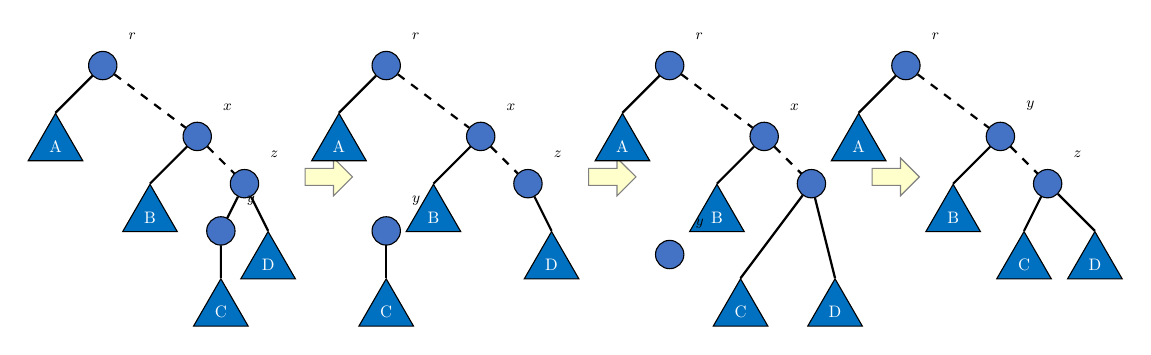
\begin{tikzpicture}[
        scale=0.6, transform shape, % <--- Thay đổi tỷ lệ ở đây nếu muốn to/nhỏ
        % --- STYLE ---
        treenode/.style={circle, draw=black, fill=nodeblue, inner sep=0pt, minimum size=0.6cm, text=white},
        subtree/.style={isosceles triangle, isosceles triangle apex angle=60, draw=black, fill=triangleblue, shape border rotate=90, minimum height=1cm, inner sep=0pt, anchor=apex, text=white},
        labeltext/.style={text=black, font=\small, above right=0.6cm}, 
        dashed_edge/.style={draw, thick, dashed, black},
        solid_edge/.style={draw, thick, black},
        steparrow/.style={single arrow, draw=black!50, fill=arrowyellow, minimum height=1cm, minimum width=0.8cm, single arrow head extend=0.15cm}
    ]

        % ==========================================
        % BƯỚC 1: BAN ĐẦU
        % ==========================================
        \begin{scope}[local bounding box=step1]
            \node[treenode] (r1) at (0,0) {}; 
            \node[labeltext] at (r1) {$r$}; 
            
            \node[subtree] (A1) at (-1,-1) {A};
            \draw[solid_edge] (r1) -- (A1.apex);
            
            \node[treenode] (x1) at (2,-1.5) {}; 
            \node[labeltext] at (x1) {$x$}; 
            \draw[dashed_edge] (r1) -- (x1);
            
            \node[subtree] (B1) at (1,-2.5) {B};
            \draw[solid_edge] (x1) -- (B1.apex);
            
            \node[treenode] (z1) at (3,-2.5) {}; 
            \node[labeltext] at (z1) {$z$}; 
            \draw[dashed_edge] (x1) -- (z1);
            
            \node[treenode] (y1) at (2.5,-3.5) {}; 
            \node[labeltext] at (y1) {$y$}; 
            \draw[solid_edge] (z1) -- (y1);
            
            \node[subtree] (C1) at (2.5,-4.5) {C};
            \draw[solid_edge] (y1) -- (C1.apex);
            \node[subtree] (D1) at (3.5,-3.5) {D};
            \draw[solid_edge] (z1) -- (D1.apex);
        \end{scope}

        \node[steparrow, right=0.2cm of step1] (arr1) {};

        % ==========================================
        % BƯỚC 2: TÁCH Y RA
        % ==========================================
        \begin{scope}[xshift=6cm, local bounding box=step2]
            \node[treenode] (r2) at (0,0) {}; 
            \node[labeltext] at (r2) {$r$};
            
            \node[subtree] (A2) at (-1,-1) {A};
            \draw[solid_edge] (r2) -- (A2.apex);
            
            \node[treenode] (x2) at (2,-1.5) {}; 
            \node[labeltext] at (x2) {$x$};
            \draw[dashed_edge] (r2) -- (x2);
            
            \node[subtree] (B2) at (1,-2.5) {B};
            \draw[solid_edge] (x2) -- (B2.apex);
            
            \node[treenode] (z2) at (3,-2.5) {}; 
            \node[labeltext] at (z2) {$z$};
            \draw[dashed_edge] (x2) -- (z2);
            
            % Y tách ra
            \node[treenode] (y2) at (0,-3.5) {}; \node[labeltext] at (y2) {$y$};
            \node[subtree] (C2) at (0,-4.5) {C};
            \draw[solid_edge] (y2) -- (C2.apex);
            
            \node[subtree] (D2) at (3.5,-3.5) {D};
            \draw[solid_edge] (z2) -- (D2.apex);
        \end{scope}

        \node[steparrow, right=0.2cm of step2] (arr2) {};

        % ==========================================
        % BƯỚC 3: ĐƯA Y LÊN
        % ==========================================
        \begin{scope}[xshift=12cm, local bounding box=step3]
            \node[treenode] (r3) at (0,0) {}; 
            \node[labeltext] at (r3) {$r$};
            
            \node[subtree] (A3) at (-1,-1) {A};
            \draw[solid_edge] (r3) -- (A3.apex);
            
            \node[treenode] (x3) at (2,-1.5) {}; 
            \node[labeltext] at (x3) {$x$};
            \draw[dashed_edge] (r3) -- (x3);
            
            \node[subtree] (B3) at (1,-2.5) {B};
            \draw[solid_edge] (x3) -- (B3.apex);
            
            \node[treenode] (z3) at (3,-2.5) {}; 
            \node[labeltext] at (z3) {$z$};
            \draw[dashed_edge] (x3) -- (z3);
            
            \node[treenode] (y3) at (0,-4) {}; \node[labeltext] at (y3) {$y$};
            
            \node[subtree] (C3) at (1.5,-4.5) {C};
            \node[subtree] (D3) at (3.5,-4.5) {D};
            \draw[solid_edge] (z3) -- (C3.apex);
            \draw[solid_edge] (z3) -- (D3.apex);
        \end{scope}

        \node[steparrow, right=0.2cm of step3] (arr3) {};

        % ==========================================
        % BƯỚC 4: HOÀN THÀNH
        % ==========================================
        \begin{scope}[xshift=17cm, local bounding box=step4]
            \node[treenode] (r4) at (0,0) {}; 
            \node[labeltext] at (r4) {$r$};
            
            \node[subtree] (A4) at (-1,-1) {A};
            \draw[solid_edge] (r4) -- (A4.apex);
            
            % Y thay thế X
            \node[treenode] (y4) at (2,-1.5) {}; 
            \node[labeltext] at (y4) {$y$}; 
            \draw[dashed_edge] (r4) -- (y4);
            
            \node[subtree] (B4) at (1,-2.5) {B};
            \draw[solid_edge] (y4) -- (B4.apex);
            
            \node[treenode] (z4) at (3,-2.5) {}; 
            \node[labeltext] at (z4) {$z$};
            \draw[dashed_edge] (y4) -- (z4);
            
            \node[subtree] (C4) at (2.5,-3.5) {C};
            \draw[solid_edge] (z4) -- (C4.apex);
            \node[subtree] (D4) at (4,-3.5) {D};
            \draw[solid_edge] (z4) -- (D4.apex);
        \end{scope}

    \end{tikzpicture}
\end{frame}
\begin{frame}[t]{3.5. Loại bỏ 1 nút trên BST}
    \textbf{Ví dụ tình huống 4:}
    
    \vspace{0.2cm}
    \centering
    % Dùng resizebox để ép dòng chữ dài này vừa khít slide, không bị xuống dòng
    \resizebox{0.95\textwidth}{!}{
        \large 
        \textcolor{nodeblue}{10, 25, 28}, \textcolor{magenta}{30}, \textcolor{textorange}{33}, \textcolor{nodeblue}{34, 35, 40, 50, 65}
        \hspace{0.5cm} $\Rightarrow$ \hspace{0.5cm}
        \textcolor{nodeblue}{10, 25, 28}, \textcolor{textorange}{33}, \textcolor{nodeblue}{34, 35, 40, 50, 65}
    }
    
    \vspace{0.5cm}
    
    \begin{tikzpicture}[
        scale=0.8, transform shape,
        level distance=1.2cm,
        sibling distance=3cm,
        level 2/.style={sibling distance=1.5cm},
        level 3/.style={sibling distance=1.5cm},
        % --- STYLE ---
        treenode/.style={circle, draw=black, fill=nodeblue, text=white, minimum size=0.7cm, inner sep=0pt, font=\bfseries},
        delnode/.style={treenode, fill=magenta!80}, 
        repnode/.style={treenode, fill=textorange}, 
        edge from parent/.style={draw, thick, black}
    ]

        % --- CÂY BÊN TRÁI (TRƯỚC KHI XOÁ) ---
        \node[treenode] (rootL) at (0,0) {40}
            child { node[delnode] (n30) {30} 
                child { node[treenode] {25} 
                    child { node[treenode] {10} }
                    child { node[treenode] {28} }
                }
                child { node[treenode] {35} 
                    child { node[repnode] (n33) {33} 
                        child[missing] 
                        child { node[treenode] {34} }
                    }
                    child[missing] 
                }
            }
            child { node[treenode] {65} 
                child { node[treenode] {50} }
                child[missing]
            };

        % Gạch chéo màu hồng
        \draw[magenta, line width=2pt] ($(n30.north west)+(-0.2,0.2)$) -- ($(n30.south east)+(0.2,-0.2)$);
        
        % CHỈNH SỬA VỊ TRÍ: Đưa về phía South West (below left)
        \node[below left=0.1cm and -0.2cm of n33, align=right, font=\small] (lblRep) {nút thế chỗ \\ của 30};
        \draw[->, thick] (lblRep) -- (n33);

        % --- MŨI TÊN CHUYỂN ĐỔI ---
        \node[single arrow, draw=black!50, fill=yellow!40, minimum height=1.5cm] at (5,-1.5) {};

        % --- CÂY BÊN PHẢI (SAU KHI XOÁ) ---
        \begin{scope}[xshift=9cm]
            \node[treenode] (rootR) at (0,0) {40}
                child { node[repnode] {33} 
                    child { node[treenode] {25} 
                        child { node[treenode] {10} }
                        child { node[treenode] {28} }
                    }
                    child { node[treenode] {35} 
                        child { node[treenode] {34} } 
                        child[missing] 
                    }
                }
                child { node[treenode] {65} 
                    child { node[treenode] {50} }
                    child[missing]
                };
        \end{scope}

    \end{tikzpicture}
\end{frame}
\begin{frame}[fragile]{3.5. Cài đặt Xóa nút}
    \begin{columns}
        \begin{column}{0.55\textwidth}
            \begin{minted}[fontsize=\tiny]{c}
TreeNode* delete(TreeNode* T, float x) {
    if (T == NULL) return NULL;
    if (x < T->key) T->leftPtr = delete(T->leftPtr, x);
    else if (x > T->key) T->rightPtr = delete(T->rightPtr, x);
    else { // Found
        if (T->leftPtr && T->rightPtr) { // 2 children
            TreeNode* tmp = find_min(T->rightPtr);
            T->key = tmp->key;
            T->rightPtr = delete(T->rightPtr, T->key);
        } else { // 1 or 0 child
            TreeNode* tmp = T;
            if (T->leftPtr == NULL) T = T->rightPtr;
            else if (T->rightPtr == NULL) T = T->leftPtr;
            free(tmp);
        }
    }
    return T;
}
            \end{minted}
        \end{column}
        \begin{column}{0.4\textwidth}
            \textbf{Độ phức tạp:}
            \begin{itemize}
                \item Trung bình: $O(\log n)$
                \item Tệ nhất (cây lệch): $O(n)$
            \end{itemize}
        \end{column}
    \end{columns}
\end{frame}

% --- Traversal ---
\subsection{Duyệt theo thứ tự giữa}
\begin{frame}[t]{3.6. Duyệt theo thứ tự giữa}
    \vspace{0.2cm}
    \centering
    
    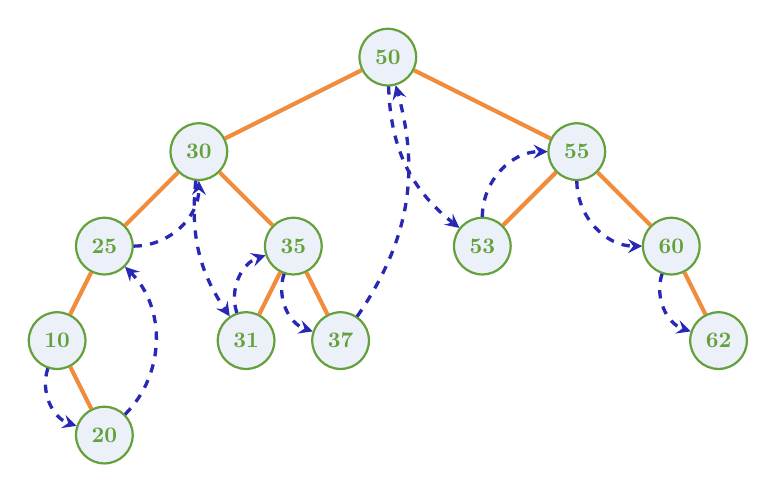
\begin{tikzpicture}[
        scale=0.8, transform shape,
        % Cấu hình cây
        level distance=1.5cm,
        level 1/.style={sibling distance=6cm},
        level 2/.style={sibling distance=3cm},
        level 3/.style={sibling distance=1.5cm},
        % Style cho node
        treenode/.style={
            circle, draw=nodetext, thick, fill=nodeblue!10, 
            text=nodetext, font=\bfseries, minimum size=0.9cm, inner sep=0pt
        },
        % Style cho cạnh cây
        edge from parent/.style={draw, edgeorange, line width=1.5pt},
        % Style cho đường duyệt (Mũi tên xanh)
        patharrow/.style={
            ->, >=stealth, pathblue, line width=1.2pt, dashed
        }
    ]

        % --- 1. VẼ CÂY ---
        \node[treenode] (n50) {50}
            child { node[treenode] (n30) {30}
                child { node[treenode] (n25) {25}
                    child { node[treenode] (n10) {10} 
                        child[missing]
                        child { node[treenode] (n20) {20} }
                    }
                    child[missing]
                }
                child { node[treenode] (n35) {35}
                    child { node[treenode] (n31) {31} }
                    child { node[treenode] (n37) {37} }
                }
            }
            child { node[treenode] (n55) {55}
                child { node[treenode] (n53) {53} }
                child { node[treenode] (n60) {60} 
                    child[missing]
                    child { node[treenode] (n62) {62} }
                }
            };

        % --- 2. VẼ MŨI TÊN DUYỆT (Từng bước) ---
        % Thứ tự: 10 -> 20 -> 25 -> 30 -> 31 -> 35 -> 37 -> 50 -> 53 -> 55 -> 60 -> 62
        
        \draw[patharrow, bend right=45] (n10) to (n20);
        \draw[patharrow, bend right=45] (n20) to (n25);
        \draw[patharrow, bend right=45] (n25) to (n30);
        \draw[patharrow, bend right=20] (n30) to (n31); % Nhảy sang nhánh phải của 30
        \draw[patharrow, bend left=45]  (n31) to (n35); % Vòng lên cha
        \draw[patharrow, bend right=45] (n35) to (n37);
        \draw[patharrow, bend right=25] (n37) to (n50); % Nhảy lên gốc
        \draw[patharrow, bend right=25] (n50) to (n53); % Xuống nhánh phải lớn
        \draw[patharrow, bend left=45]  (n53) to (n55);
        \draw[patharrow, bend right=45] (n55) to (n60);
        \draw[patharrow, bend right=45] (n60) to (n62);

    \end{tikzpicture}

    \vspace{0.3cm}
    
    % --- KẾT QUẢ ---
    \textbf{\textcolor{textdark}{Thứ tự duyệt (Tăng dần):}} \\
    \textcolor{resultred}{10 $\rightarrow$ 20 $\rightarrow$ 25 $\rightarrow$ 30 $\rightarrow$ 31 $\rightarrow$ 35 $\rightarrow$ 37 $\rightarrow$ 50 $\rightarrow$ 53 $\rightarrow$ 55 $\rightarrow$ 60 $\rightarrow$ 62}

\end{frame}

\begin{frame}{3.6. Duyệt và Tổng kết}
    \textbf{Duyệt giữa (In-order Traversal):}
    \begin{itemize}
        \item Duyệt con trái $\to$ Duyệt gốc $\to$ Duyệt con phải.
        \item \textbf{Kết quả:} Dãy khóa được sắp xếp tăng dần.
        \item Độ cao trung bình của BST là: h = O(log n)
    \end{itemize}
        

    \vspace{0.5cm}
    \textbf{Tổng kết độ phức tạp (Trung bình):}
    \begin{table}[]
        \centering
        \begin{tabular}{lc}
            \toprule
            \textbf{Thao tác} & \textbf{Độ phức tạp} \\
            \midrule
            Tìm kiếm (Search) & $O(\log n)$ \\
            Chèn (Insertion) & $O(\log n)$ \\
            Xóa (Deletion) & $O(\log n)$ \\
            Tìm Min/Max & $O(\log n)$ \\
            Sắp xếp (BST Sort) & $O(n \log n)$ \\
            \bottomrule
        \end{tabular}
    \end{table}
\end{frame}

% --- Thank You ---
{\HUSTUseBackground{theme_hust_oneside.pdf}
\begin{frame}[plain]
    \ifdefstring{\insertaspectratio}{169}{
        \placecontent{0.355\paperwidth}{0.410\paperheight}{0.640\paperwidth}{
            \color{HUSTRed}\bfseries\fontsize{28pt}{36pt}\selectfont\centering
            THANK YOU!
        }
    }{}
\end{frame}
}

\end{document}